% !TeX spellcheck = en_GB
\documentclass[english,11pt,aspectratio=1610,xcolor=table]{beamer}
% !TeX root = ../defense.tex
% packages
\usepackage{babel}
\usepackage[utf8]{inputenc}
\usepackage[scaled=0.86]{beramono}
\usepackage{helvet}
\usepackage[T1]{fontenc}

\usepackage{eurosym}
\usepackage[output-decimal-marker={,},per-mode=symbol,exponent-product={\cdot},retain-unity-mantissa=false]{siunitx}
\usepackage{csquotes}
\usepackage{tikz}
\usepackage{pgfplots}
\usepackage{listings}
\usepackage{mathtools}
\usepackage{textcomp}
\usepackage[version=4]{mhchem}
\usepackage{bm}
\usepackage{tabu}
\usepackage{appendixnumberbeamer}

% tikz libraries
\usetikzlibrary{arrows.meta}
\usetikzlibrary{calc}
\usetikzlibrary{decorations.pathreplacing}
\usetikzlibrary{positioning}
\usetikzlibrary{shapes}
\usetikzlibrary{arrows}
\usetikzlibrary{positioning}

% pgfplots libraries
\usepgfplotslibrary{fillbetween}



\tikzstyle{terminator} = [rectangle, draw, text centered, rounded corners, minimum height=2em]
\tikzstyle{process} = [rectangle, draw, text centered, minimum height=2em]
\tikzstyle{decision} = [diamond, draw, text centered, minimum height=2em]
\tikzstyle{data}=[trapezium, draw, text centered, trapezium left angle=60, trapezium right angle=120, minimum height=2em]
\tikzstyle{connector} = [draw, -latex']
% !TeX root = ../defense.tex
% colors
% tum main colors
\definecolor{tumblue}{RGB}{0, 101, 189}
\definecolor{tumblack}{RGB}{0, 0, 0}
\definecolor{tumwhite}{RGB}{255, 255, 255}

% tum blue tones (shades !85, !70, !55 allowed)
\definecolor{tumdarkerblue}{RGB}{0, 51, 89}
\definecolor{tumdarkblue}{RGB}{0, 82, 147}
\definecolor{tummidblue}{RGB}{0, 115, 207}
\definecolor{tumlightblue}{RGB}{100, 160, 200}
\definecolor{tumlighterblue}{RGB}{152, 198, 234}

% tum grey tones
\definecolor{tumdarkergrey}{RGB}{44, 44, 45}
\definecolor{tumdarkgrey}{RGB}{88, 88, 90}
\definecolor{tumgrey}{RGB}{156, 157, 159}
\definecolor{tumlightgrey}{RGB}{217, 218, 219}
\definecolor{tumlightergrey}{RGB}{235, 236, 237}

% tum accent colors (shades !85, !70, !55 allowed)
\definecolor{tumorange}{RGB}{227,114,34}
\definecolor{tumgreen}{RGB}{162,173,0}
\definecolor{tumivory}{RGB}{218,215,203}

% tum extended palette (shades !85, !70, !55 allowed)
\definecolor{tumviolet}{RGB}{105,8,90}
\definecolor{tumdarkviolet}{RGB}{15,27,95}
\definecolor{tumturquois}{RGB}{0,119,138}
\definecolor{tumdarkgreen}{RGB}{0,124,48}
\definecolor{tummidgreen}{RGB}{103,154,29}
\definecolor{tumbrightyellow}{RGB}{255,220,0}
\definecolor{tumbrightorange}{RGB}{249,186,0}
\definecolor{tumbrightred}{RGB}{214,76,19}
\definecolor{tumred}{RGB}{196,7,27}
\definecolor{tumdarkred}{RGB}{156,13,22}


% tum presentation colors (styleguide, p.266)
\definecolor{tumpyellow}{RGB}{255,180,0}
\definecolor{tumporange}{RGB}{255,128,0}
\definecolor{tumpred}{RGB}{229,52,24}
\definecolor{tumpdarkred}{RGB}{202,33,63}
\definecolor{tumpblue}{RGB}{0,153,255}
\definecolor{tumpbrightblue}{RGB}{65,190,255}
\definecolor{tumpgreen}{RGB}{145,172,107}
\definecolor{tumpbrightgreen}{RGB}{181,202,130}

% custom thesis colors
\definecolor{biomass}{RGB}{0, 122, 55}
\definecolor{co2}{RGB}{160, 160, 160}
\definecolor{coal}{RGB}{100, 100, 100}
\definecolor{cool}{RGB}{0, 0, 255}
\definecolor{demand}{RGB}{25, 25, 25}
\definecolor{diesel}{RGB}{116, 66, 65}
\definecolor{gas}{RGB}{128, 64, 0}
\definecolor{elec}{RGB}{255, 170, 0}
\definecolor{heat}{RGB}{230, 112, 36}
\definecolor{hydro}{RGB}{198, 188, 240}
\definecolor{hydrogen}{RGB}{198, 188, 240}
\definecolor{imp}{RGB}{128, 128, 200}
\definecolor{lignite}{RGB}{116, 66, 65}
\definecolor{nuclear}{RGB}{192, 34, 16}
\definecolor{oil}{RGB}{116, 66, 65}
\definecolor{overproduction}{RGB}{190, 0, 99}
\definecolor{slack}{RGB}{163, 74, 130}
\definecolor{solar}{RGB}{243, 174, 0}
\definecolor{storage}{RGB}{60, 36, 154}
\definecolor{wind}{RGB}{122, 179, 225}
\definecolor{stock}{RGB}{222, 222, 222}

% custom building type colors
\definecolor{basin}{RGB}{110, 75, 56}
\definecolor{chapel}{RGB}{177, 121, 91}
\definecolor{church}{RGB}{177, 121, 91}
\definecolor{commercial}{RGB}{129, 162, 190}
\definecolor{farm}{RGB}{202, 178, 214}
%\definecolor{garage}{RGB}{253, 191, 111}
\definecolor{greenhouse}{RGB}{255, 127, 0}
%\definecolor{hospital}{RGB}{129, 221, 190}
\colorlet{hospital}{tumturquois}
%\definecolor{hotel}{RGB}{227, 26, 28}
\colorlet{hotel}{tumorange!50}
\definecolor{house}{RGB}{181, 189, 104}
\definecolor{industrial}{RGB}{240, 198, 116}
\definecolor{office}{RGB}{129, 162, 190}
%\definecolor{public}{RGB}{129, 162, 190}
\definecolor{residential}{RGB}{181, 189, 104}
\definecolor{restaurant}{RGB}{227, 26, 28}
%\definecolor{retail}{RGB}{129, 162, 190}
\definecolor{school}{RGB}{29, 103, 214}
%\definecolor{warehouse}{RGB}{98, 134, 6}
\colorlet{warehouse}{tumgrey!50}
\colorlet{garage}{tumgrey!75}
\colorlet{public}{commercial!50}
\colorlet{other}{tumgrey}
\colorlet{retail}{commercial!75}

\usepackage{contour}

\usepackage{amsmath}
% Definition of \boxed in amsmath.sty:
% \newcommand{\boxed}[1]{\fbox{\m@th$\displaystyle#1$}}

\usepackage{xcolor}
% Syntax: \colorboxed[<color model>]{<color specification>}{<math formula>}
\newcommand*{\colorboxed}{}
\def\colorboxed#1#{%
	\colorboxedAux{#1}%
}
\newcommand*{\colorboxedAux}[3]{%
	% #1: optional argument for color model
	% #2: color specification
	% #3: formula
	\begingroup
	\colorlet{cb@saved}{.}%
	\color#1{#2}%
	\boxed{%
		\color{cb@saved}%
		#3%
	}%
	\endgroup
}
\input{tex/setup-settings}

\usepackage[normalem]{ulem}

\newcommand{\der}{\mathrm{d}}

\usetheme{JD}
\beamertemplatenavigationsymbolsempty

% header fields: usage
% \field
%     [short form (footline)]
%     {long form on title page}
%
\title
    [SGWB detection with TDA]
    {Detection of Stochastic Gravitational Wave Background\\ Based on Topological Data Analysis}

\subtitle{M.Sc. Thesis defense} % short version unused by this template
\author
    [A. Salehi]
    {Ali Salehi}
\institute
    [\hypersetup{urlcolor=jdgrey}%
     \href{http://www.ccg.sbu.ac.ir/}{CCG} %
     \href{http://www.sbu.ac.ir}{SBU}]
    {Computational Cosmology Group\\
     Department of Physics\\%
     Shahid Beheshti University}
\date
    [2023/06]
    {28 Shahrivar 2023}

%\logo{
\includegraphics[width=1cm]{logo}}
\titlegraphic{
\includegraphics[width=2cm]{logo}}

%\titlegraphic{%
%\begin{picture}(0,0)
%		\put(-40,-150){\makebox(0,0)[rt]{
\includegraphics[width=2cm]{logo}}}
%\end{picture}}
%\AtBeginSection[]{
%	\begin{frame}{Talk Overview}
%		\tableofcontents[currentsection]
%	\end{frame}
%	\frame{\sectionpage}
%}


\begin{document}

\maketitle

\begin{frame}{Overview}
\begin{center}
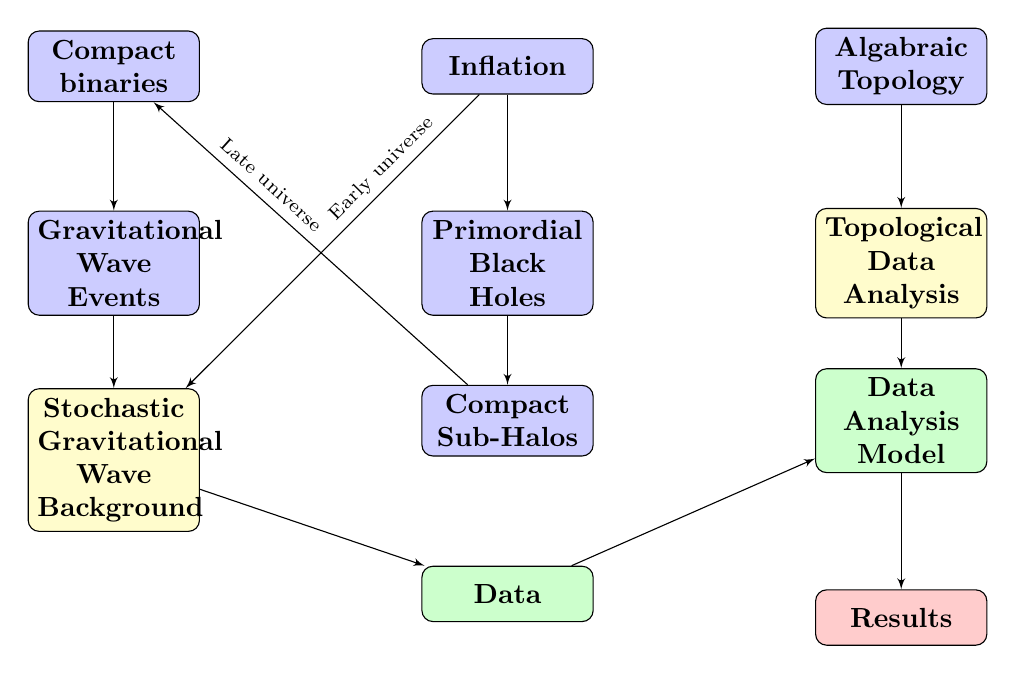
\begin{tikzpicture}%[
	%node distance=4.5em and .75cm,font=\small
	%]
	\node[terminator, fill=yellow!20] (SGWB) at (-7, 2) {
		\begin{minipage}{.16\textwidth}
			\centering
			\textbf{Stochastic\\ Gravitational Wave\\ Background}
		\end{minipage}};

	\node[terminator, fill=yellow!20] (TDA) at (3, 4.5) {
		\begin{minipage}{.16\textwidth}
			\centering
			\textbf{Topological Data\\ Analysis}
		\end{minipage}};
\uncover<2-12>{
	\node[terminator, fill=blue!20] (Inf) at (-2, 7) {
		\begin{minipage}{.16\textwidth}
			\centering
			\textbf{Inflation}
		\end{minipage}};
}
\uncover<2-5>{
	\path [connector] (Inf) -- (SGWB);
	\node [draw=none, rotate=45] at (-3.6, 5.7) {\scriptsize Early universe};
}
\uncover<3-12>{
	\node[terminator, fill=blue!20] (GW) at (-7, 4.5) {
		\begin{minipage}{.16\textwidth}
			\centering
			\textbf{Gravitational Wave\\ Events}
		\end{minipage}};		
	\path [connector] (GW) -- (SGWB);
}
\uncover<4-12>{
	\node[terminator, fill=blue!20] (BBH) at (-7, 7) {
		\begin{minipage}{.16\textwidth}
			\centering
			\textbf{Compact binaries}
		\end{minipage}};
	\path [connector] (BBH) -- (GW);
}

\uncover<5-12>{	
	\node[terminator, fill=blue!20] (PBH) at (-2, 4.5) {
		\begin{minipage}{.16\textwidth}
			\centering
			\textbf{Primordial\\ Black Holes}
		\end{minipage}};
	\path [connector] (Inf) -- (PBH);
}
\uncover<6-12>{
	\node[terminator, fill=blue!20] (Clust) at (-2, 2.5) {
		\begin{minipage}{.16\textwidth}
			\centering
			\textbf{Compact\\ Sub-Halos}
		\end{minipage}};
	\path [connector] (PBH) -- (Clust);
}
\uncover<7-12>{
	\path [connector] (Clust) -- (BBH);
	\node [draw=none, rotate=-42] at (-5, 5.5) {\scriptsize Late universe};
}
\uncover<8-12>{
	\node[terminator, fill=blue!20] (Top) at (3, 7) {
		\begin{minipage}{.16\textwidth}
			\centering
			\textbf{Algabraic\\ Topology}
		\end{minipage}};
	\path [connector] (Top) -- (TDA);
}
\uncover<9-12>{
	\node[terminator, fill=green!20] (Ana) at (3, 2.5) {
		\begin{minipage}{.16\textwidth}
			\centering
			\textbf{Data Analysis\\ Model}
		\end{minipage}};
	\path [connector] (TDA) -- (Ana);
}
\uncover<10-12>{
	\node[terminator, fill=green!20] (Dat) at (-2, 0.3) {
		\begin{minipage}{.16\textwidth}
			\centering
			\textbf{Data}
		\end{minipage}};
	\path [connector] (SGWB) -- (Dat);
}
\uncover<11-12>{
	\path [connector] (Dat) -- (Ana);
}
\uncover<12>{
	\node[terminator, fill=red!20] (Res) at (3, 0) {
		\begin{minipage}{.16\textwidth}
			\centering
			\textbf{Results}
		\end{minipage}};
	\path [connector] (Ana) -- (Res);
}

\end{tikzpicture}
\end{center}
\end{frame}


\begin{frame}{Outline}
    \tableofcontents
\end{frame}

% !TeX root = ../defense.tex

\section{Gravitational Waves}
\frame{\sectionpage}

\begin{frame}{Where do the gravitational waves come from?}
\begin{columns}
\begin{column}{.4\linewidth}
Einstein Equations:
\begin{align*}
	\uncover<+->{
		G_{\mu\nu} &= \frac{8 \pi G}{c^4} T_{\mu\nu}\\
	}
	\uncover<+->{
		G_{\mu\nu} &= G_{\mu\nu} (g_{\mu\nu}, \dot{g}_{\mu\nu}, \ddot{g}_{\mu\nu}) \\
		\uncover<+->{&= R_{\mu\nu} - \frac{1}{2} g_{\mu\nu} R}
	}
\end{align*}
\begin{align*}
	\uncover<+->{
		&R = g^{\mu\nu} R_{\mu\nu}\\ 
	}
	\uncover<+->{
		&R_{\mu\nu} = R^{\sigma}_{~\mu\sigma\nu}\\
	}
	\uncover<+->{
		&R^{\sigma}_{~\mu\rho\nu} = {R^{\sigma}}_{\mu\rho\nu} (\dot{g}_{\mu\nu}, \ddot{g}_{\mu\nu})
	}
\end{align*}
\vspace*{\fill}
\end{column}
\hspace*{\fill}
\begin{column}{.4\linewidth}
\uncover<+->{Einstein Field Equations:}
\begin{align*}
	\uncover<+->{
		\text{}
		&G_{\mu\nu} = 0
	}
\end{align*}
\begin{align*}
	\uncover<+->{
		\text{if:\quad}
		&g_{\mu\nu} = \eta_{\mu\nu} \text{\quad(everywhere)}\\
	}
	\uncover<+->{
		\therefore\quad &R_{\mu\nu} = 0 \implies G_{\mu\nu} = 0
	}
\end{align*}
\uncover<+->{First order variations:}
\begin{align*}
	\uncover<+->{
		\text{if:\quad}
		g_{\mu\nu} &= \eta_{\mu\nu} + \varepsilon h_{\mu\nu}\\
	}
	\uncover<+->{
		&~~\vdots \\
	}
	\uncover<+->{
		\therefore \quad \Aboxed{\Box h_{\mu\nu} &= 0}
	}
\end{align*}
%\vfill
\end{column}
\end{columns}
\end{frame}

\begin{frame}{But what are gravitational waves?}
\begin{columns}
\begin{column}{0.5\linewidth}
\begin{align*}
	\uncover<+->{
		&\Box h_{\mu\nu} = 0 \\~\\
		\uncover<+->{\rightarrow \quad &\frac{1}{c^2}\frac{\partial^2}{\partial t^2}h_A = \left(\frac{\partial^2}{\partial x^2} + \frac{\partial^2}{\partial y^2} + \frac{\partial^2}{\partial z^2} \right) h_A\\
		&\scriptstyle{(T = +, \times)}}\\
	}
\end{align*}
\uncover<4->{In Transverse-Traceless Guage:}\\
\begin{align*}
	\uncover<5->{
		h_{\mu\nu} = 
		\begin{pmatrix}
			0  & 0         & 0         & 0 \\
			0  & h_+       & h_\times  & 0  \\
			0  & h_\times  & -h_+      & 0  \\
			0  & 0         & 0         & 0 
		\end{pmatrix}
	}
\end{align*}
\end{column}
\begin{column}{0.5\linewidth}
\vfill
\uncover<3->{
	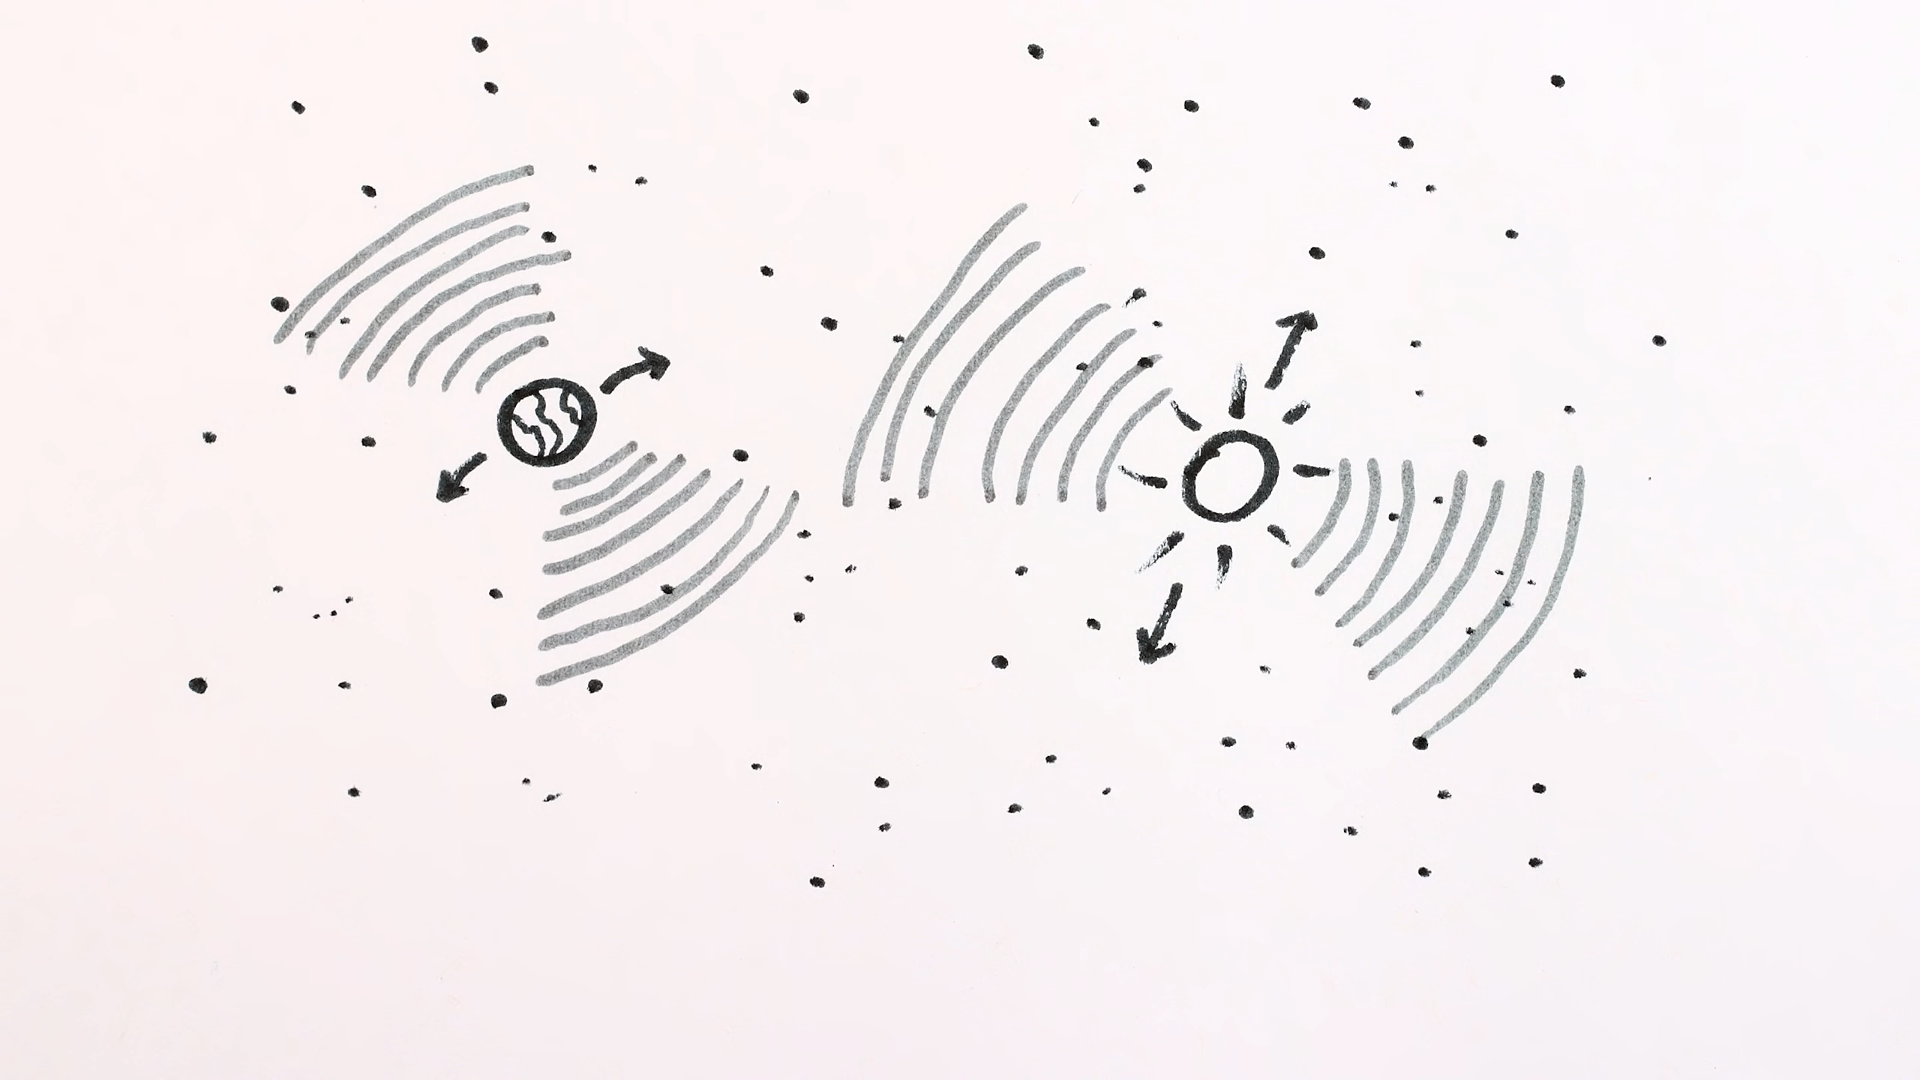
\includegraphics[width=\linewidth]{img/GW-minutephysics}
	\textcolor{gray}{\fontsize{7.5}{10}\selectfont Image credit: \href{https://www.youtube.com/channel/UCUHW94eEFW7hkUMVaZz4eDg}{Youtube: minutephysics}}
}
\end{column}
\end{columns}
\end{frame}

\begin{frame}{Polarizations are the signature of gravitational waves}
\begin{columns}
\begin{column}{.7\linewidth}
	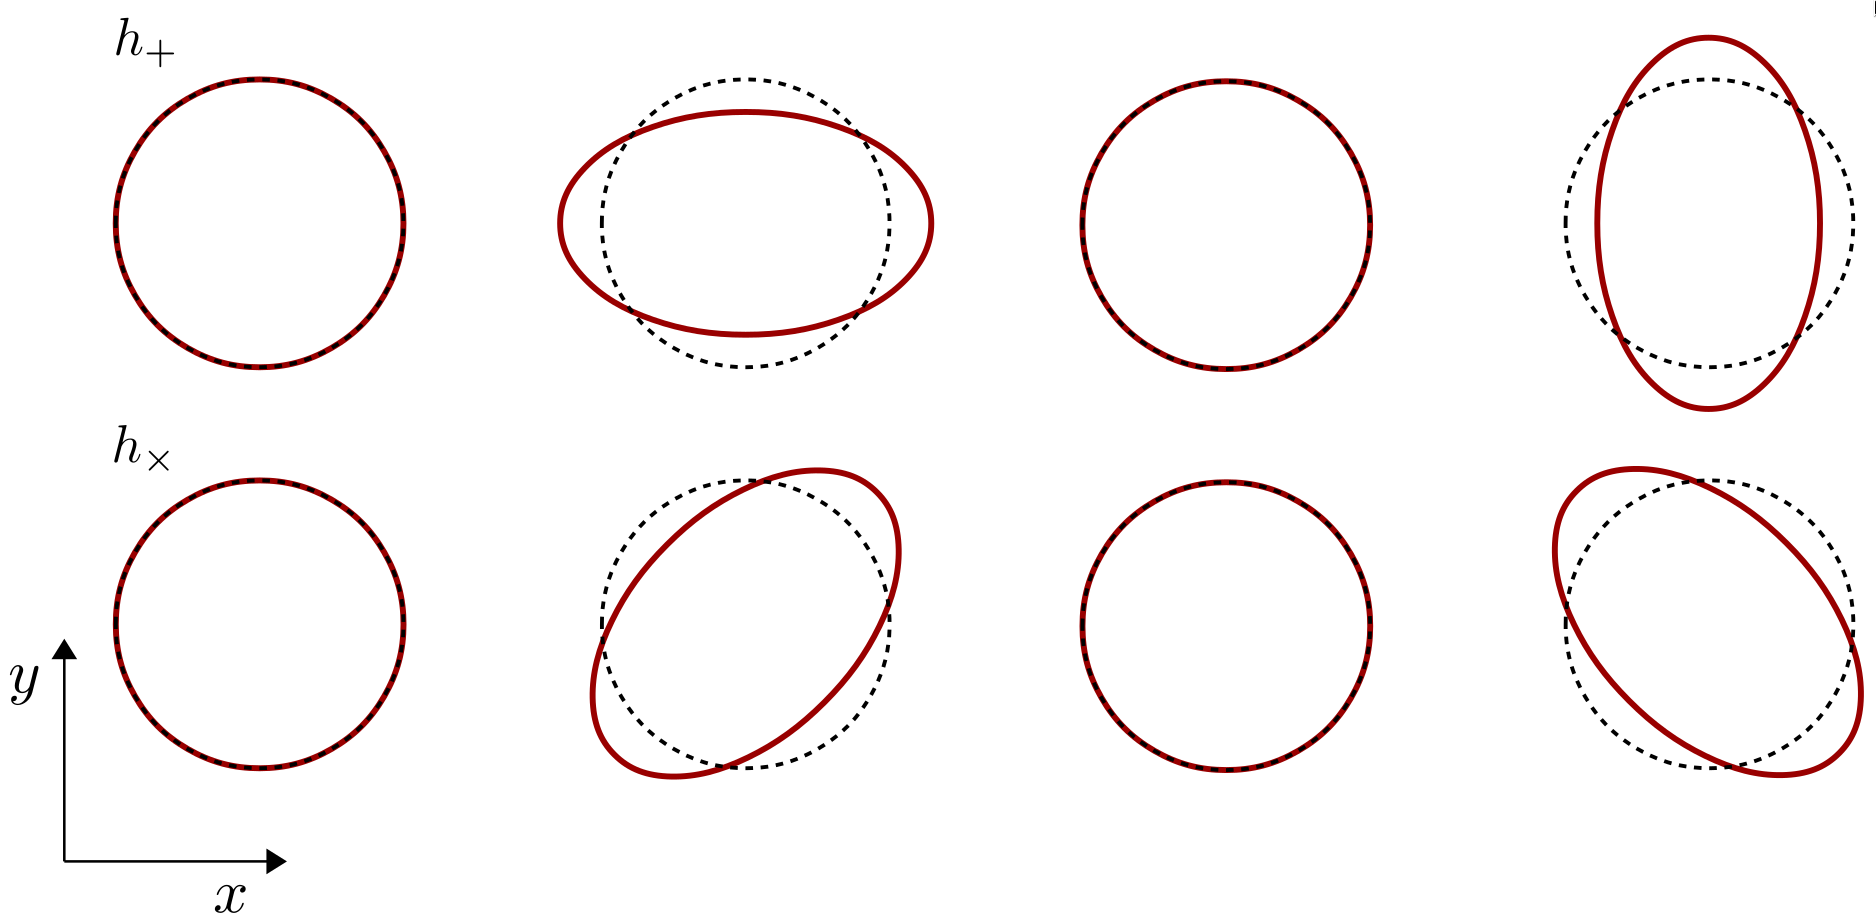
\includegraphics[width=\linewidth]{img/polarization}
\end{column}
\begin{column}{.3\linewidth}
	\textcolor{gray}{\fontsize{7.5}{10}\selectfont Image credit:\\ \href{https://www.elsevier.com/books/modern-cosmology/dodelson/978-0-12-815948-4}{S. Dodelson, F. Schmidt, Modern Cosmology}}
	\vspace*{\fill}
\end{column}
\end{columns}
\vspace*{\fill}
\uncover<2->{Other Gravitational wave features:\\}
\begin{itemize}
	\item<3-> They can not be detected locally (Because of equivalance principal)
	\item<4-> They travel at the speed of light
\end{itemize}
\end{frame}


\begin{frame}{Sources of Gravitational Waves}
\begin{columns}
\begin{column}{.6\linewidth}
\uncover<+->{Burst:}
\begin{itemize}
	\item<+-> Supernovae \\~\\
\end{itemize}
\uncover<4->{Continuous and Inspiral:}
\begin{itemize}
	\item<5-> Binary mergers (NS, SBH, PBH, SMBH, ...)
	\item<6-> Neutron stars with deformities \\~\\
\end{itemize}
\uncover<8->{Stochastic:}
\begin{itemize}[<9->]
	\item<9-> Primordial tensor perturbations
	\item<10-> Secondary tensor perturbations
	\item<11-> Topological defects (e.g. cosmic strings)
	\item<12-> Superposition of the other types
\end{itemize}
\end{column}
\begin{column}{.4\linewidth}
\uncover<3->{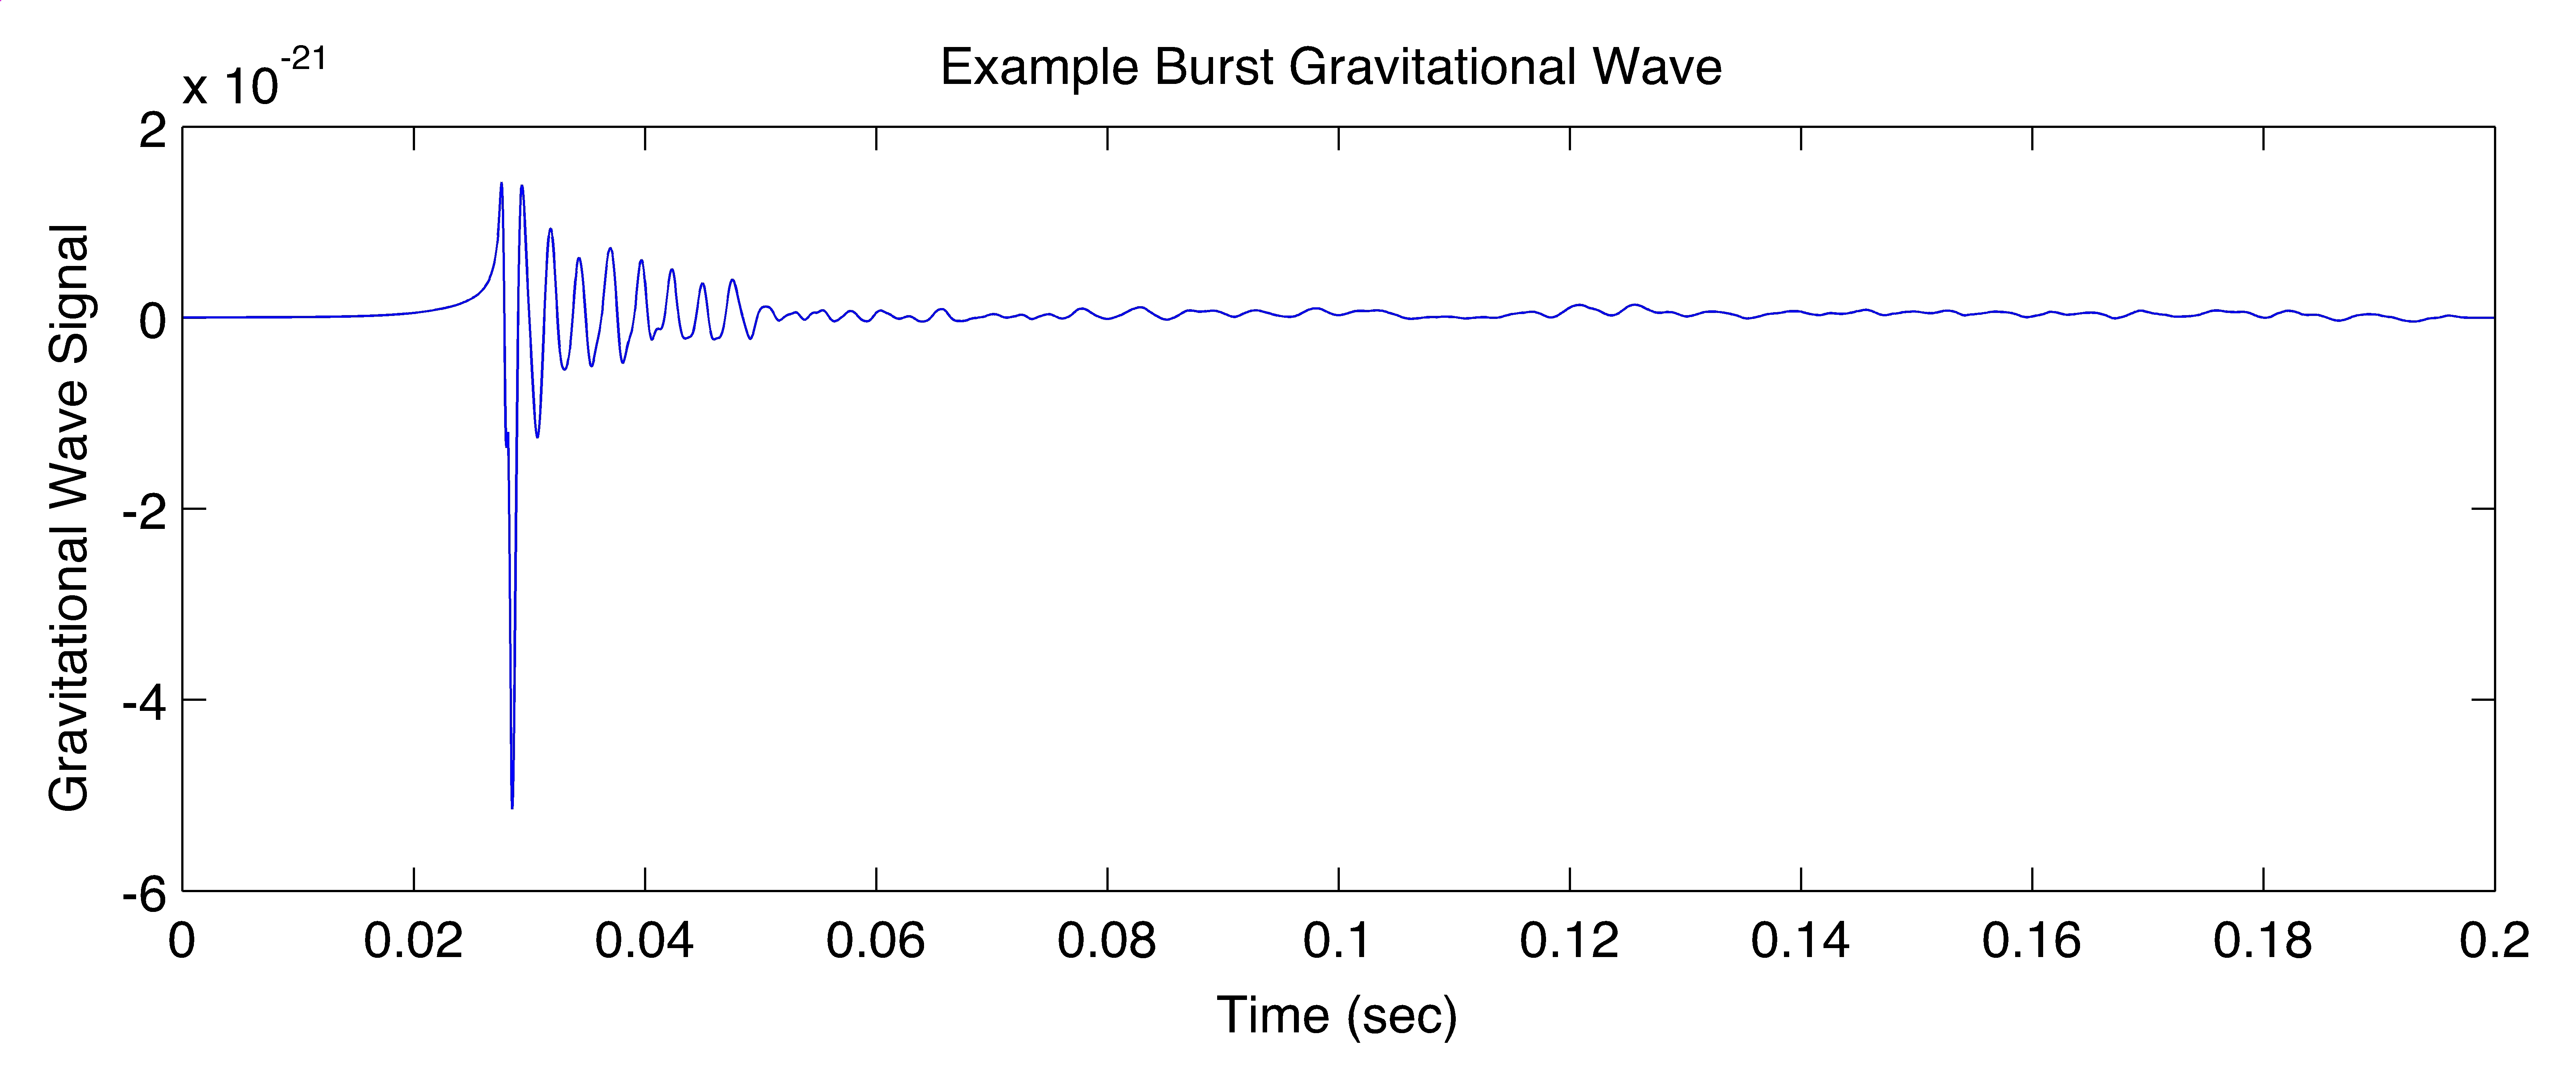
\includegraphics[width=\linewidth]{img/burst}}
\uncover<7->{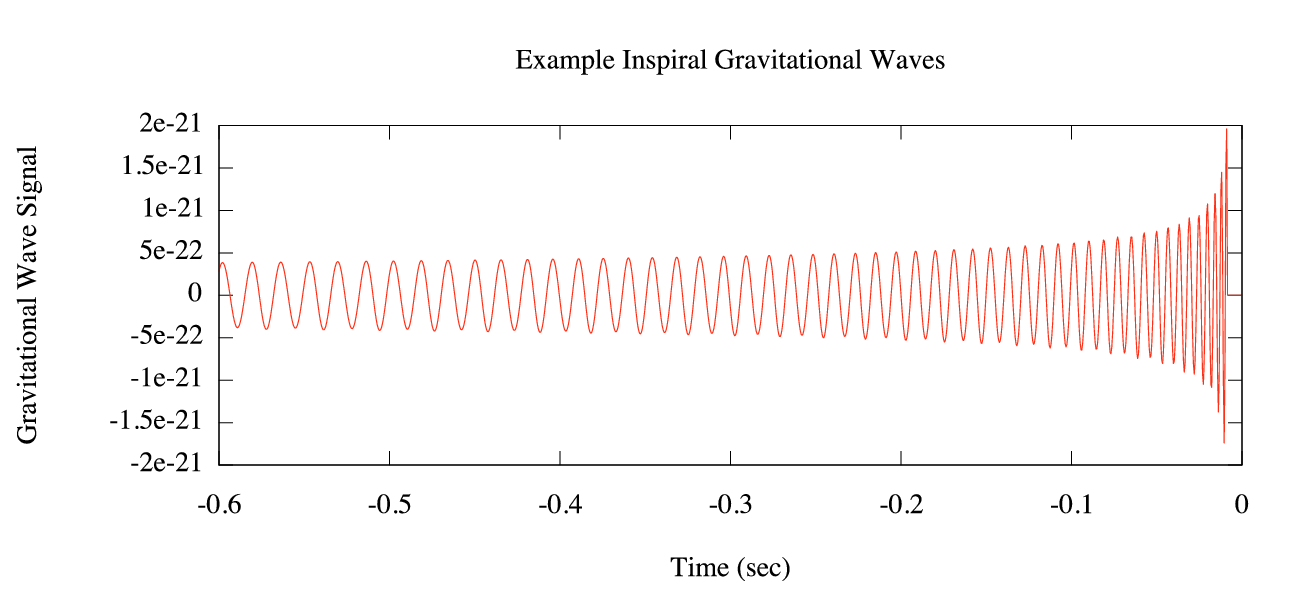
\includegraphics[width=\linewidth]{img/inspiral-0}}
\uncover<13->{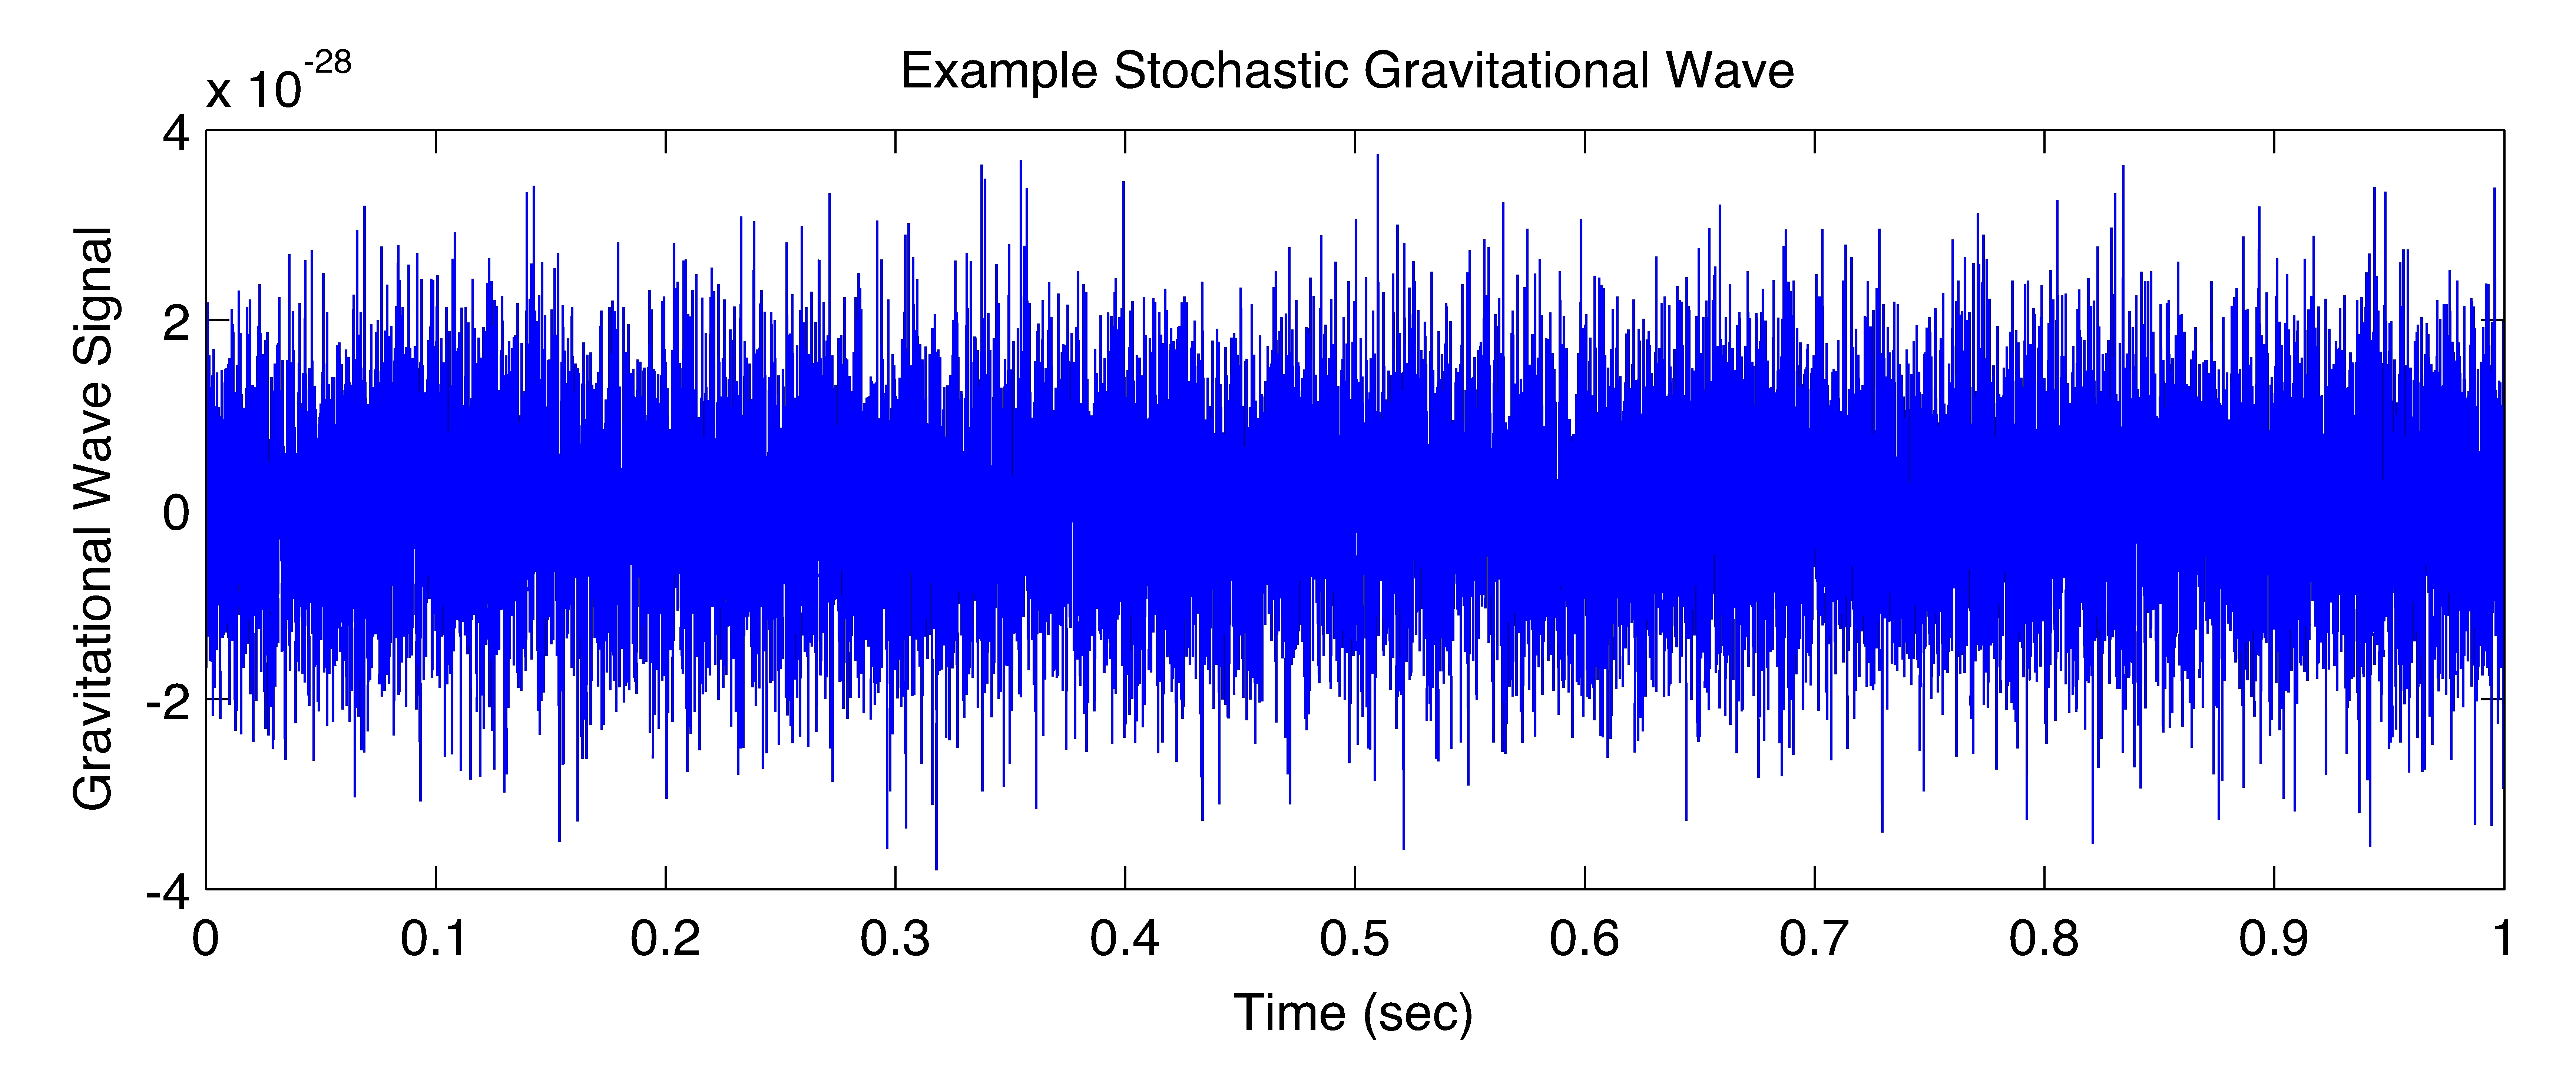
\includegraphics[width=\linewidth]{img/stochastic}}
\uncover<3->{
	\textcolor{gray}{\fontsize{4.5}{10}\selectfont Image credit:
	\href{https://www.ligo.org/science}{LIGO Scientific Collaboration}}
}
\end{column}
\end{columns}
\end{frame}

\begin{frame}{How to detect gravitational waves?}
\begin{columns}
\begin{column}{0.63\linewidth}
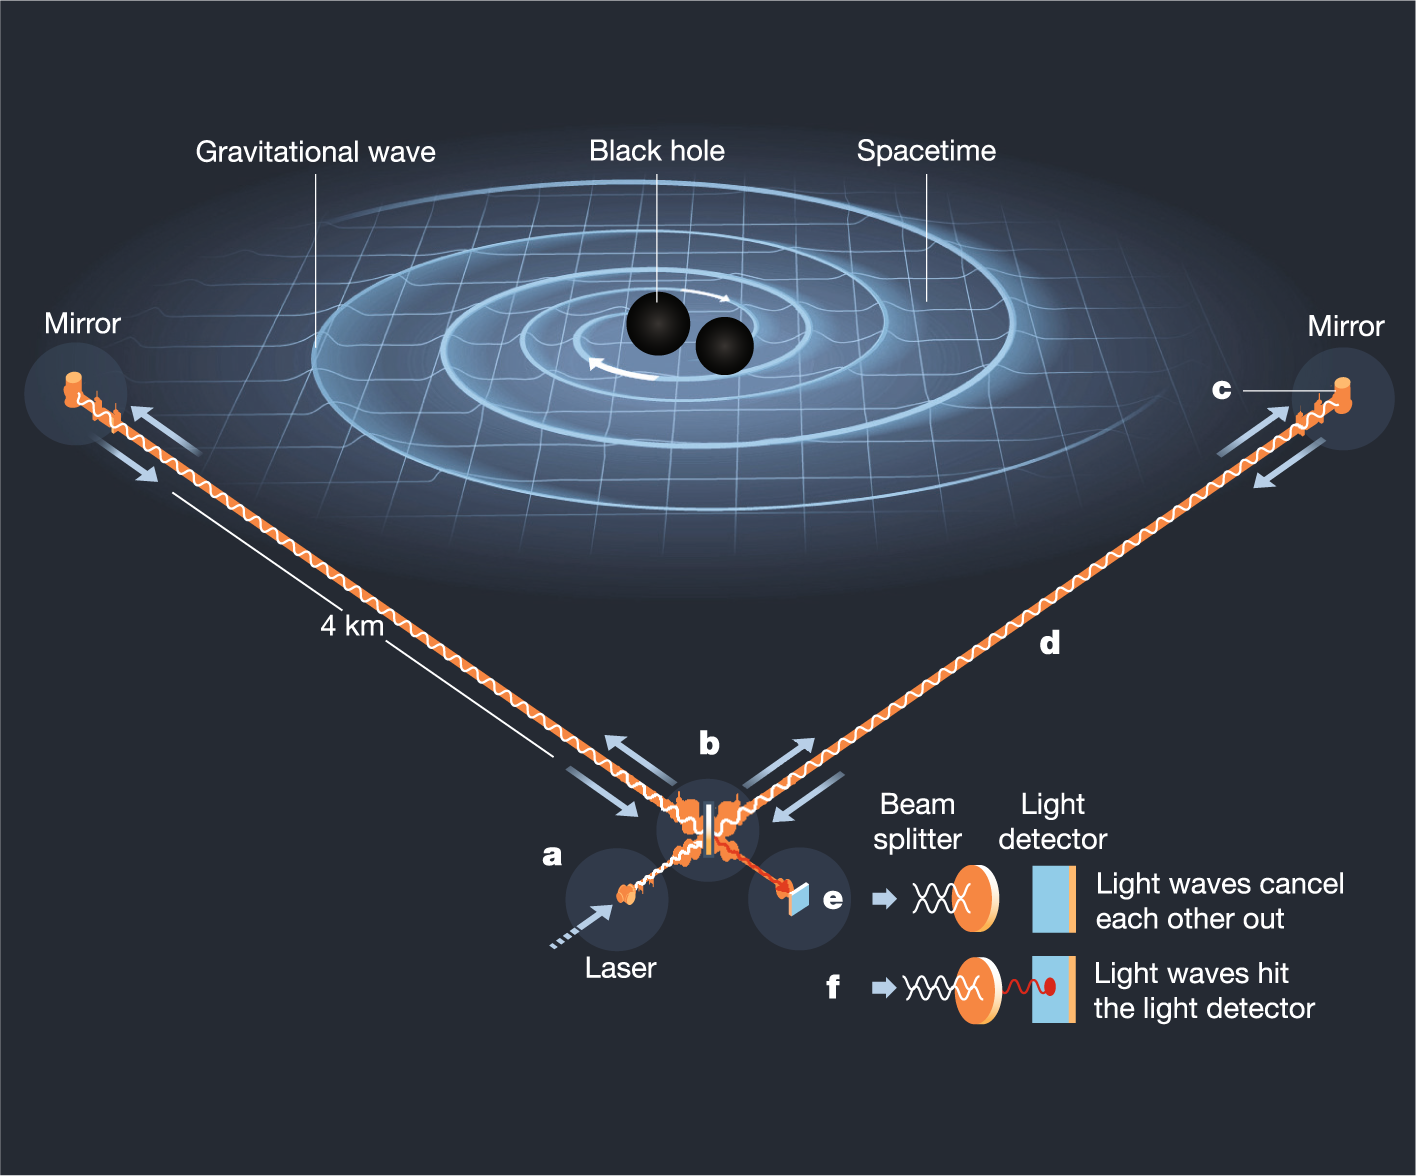
\includegraphics[width=\linewidth]{img/LIGO_setup}
\end{column}
\begin{column}{0.32\linewidth}
	\uncover<2->{
		Other detection methods:
	}
	\begin{itemize}
		\item<3-> Weber bar
		\item<4-> Pulsar timing arrays
		\item<5-> CMB B-mode
		\item<6-> Other non-direct ways
	\end{itemize}
	\vspace*{4cm}
	\textcolor{gray}{\fontsize{7.5}{10}\selectfont Image credit:
	\href{https://www.nobelprize.org/prizes/physics/2017/press-release/}{The Royal Swedish Academy of Sciences}}
\end{column}
\end{columns}
\end{frame}

\begin{frame}{Gravitational waves from black hole mergers}
\vskip 5pt
\centering
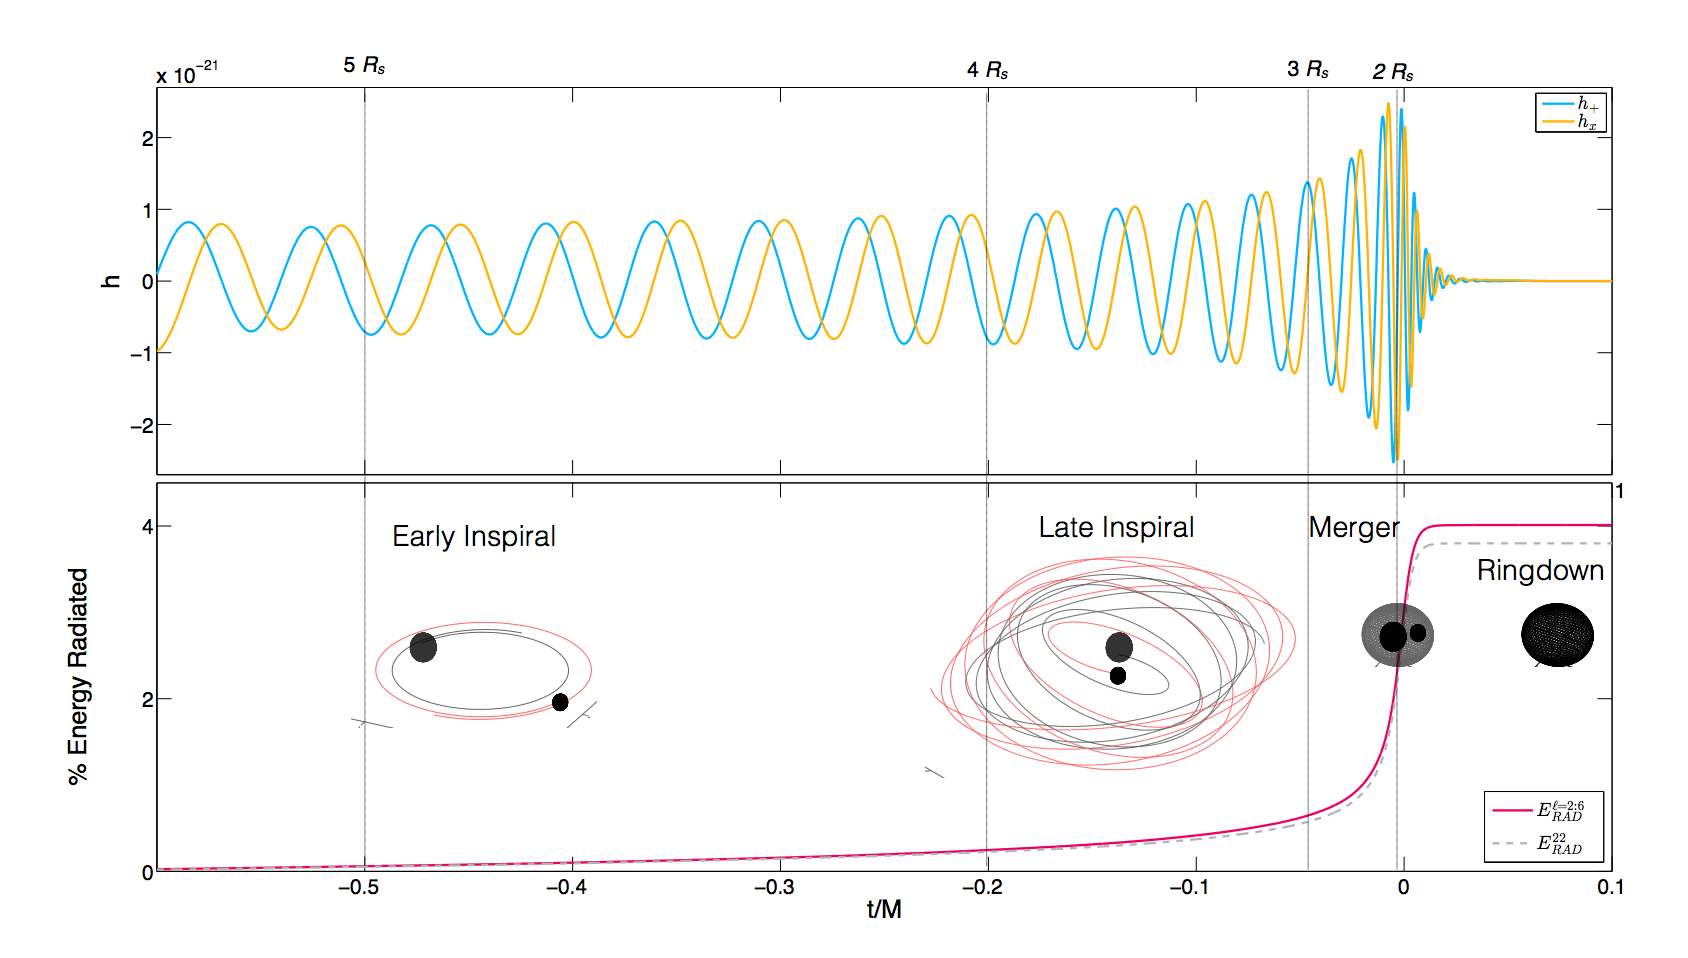
\includegraphics[width=\linewidth]{img/BBH_GT}\\
\vskip -10pt
\qquad\qquad\qquad\qquad\qquad\qquad\qquad\qquad\qquad\qquad\textcolor{gray}{\fontsize{7.5}{10}\selectfont Image credit:
\href{https://einstein.gatech.edu/catalog/}{Einstein at Georgia Tech}}
\end{frame}

\begin{frame}{Stochastic gravitational wave background}
\begin{columns}
\begin{column}{0.5\linewidth}
	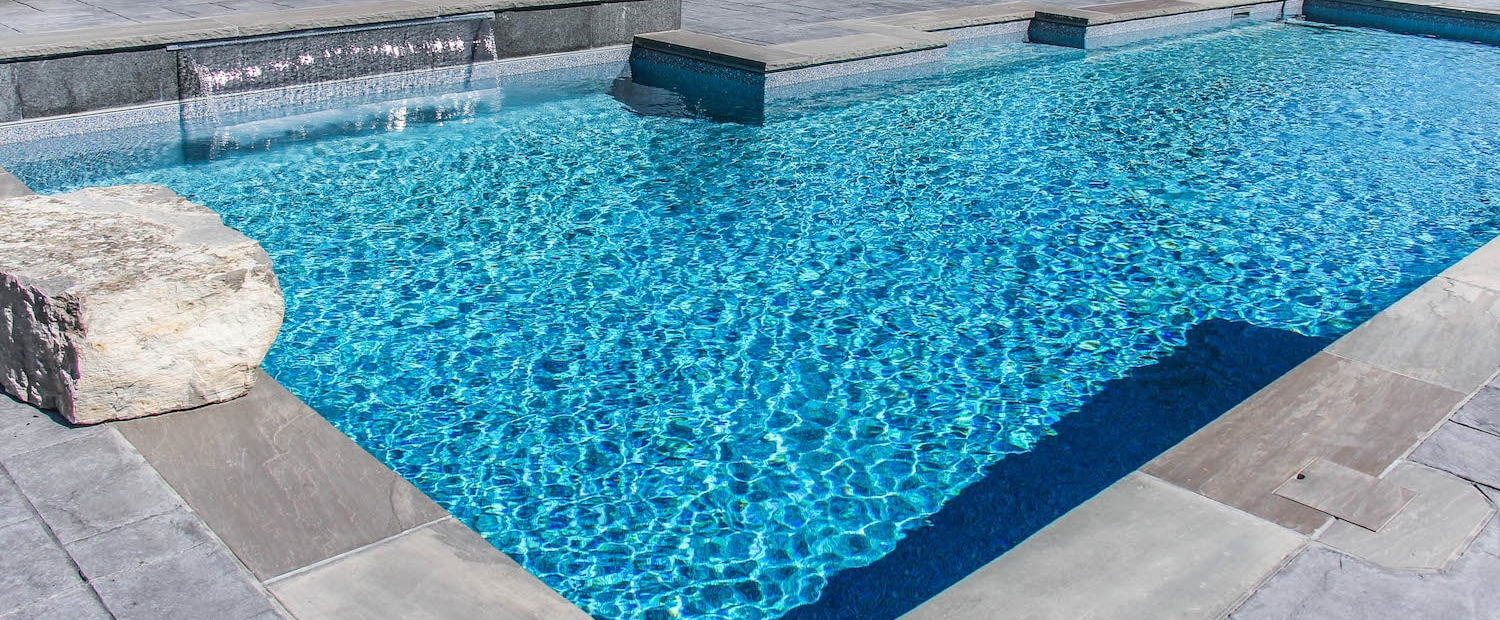
\includegraphics[width=\linewidth]{img/pool}
	\textcolor{gray}{\fontsize{6.5}{10}\selectfont Image credit: \href{http://www.megnapools.com/aqua-blue-mixnmatch}{Megna pools}}
\end{column}
\begin{column}{0.5\linewidth}
"We are like an insect sitting at the edge of a pool, trying to figure out who jumped in where and when and what's happening all over the pool."\\~\\
- Richard Feynman
\hfil
\end{column}
\end{columns}
\begin{columns}
\begin{column}{.55\linewidth}
\begin{align*}
	\uncover<2->{
		&\Omega_{SGWB} (f) = \frac{1}{\rho_c} \frac{\der \rho_{GW}(f)}{\der \ln f}\\~\\
	}
	\uncover<3->{
		h_{ab} &(t, \vec{x})\\&= \sum_{A=+,\times} \int_{-\infty}^{\infty} \der f \int_{S^2} \der \hat{\Omega} h_A(f, \hat{\Omega}) e^{2\pi i f (t - \hat{\Omega} \cdot \vec{x})} \hat{e}_{ab}^A (\hat{\Omega})
	}
\end{align*}
\end{column}
\begin{column}{.45\linewidth}
\begin{align*}
\uncover<4->{
	\langle h_A(f, \hat{\Omega})& h^*_{A^\prime}(f^\prime, \hat{\Omega}^\prime) \rangle_{\text{ens}}\\ &=\frac{\delta_{AA^\prime}}{2} \frac{\delta^{(2)} (\hat{\Omega}, \hat{\Omega}^\prime)}{4\pi} \frac{\delta(f - f^\prime)}{2} S_h(f)\\~\\
}
\uncover<5->{
	\Aboxed{&\Omega_{SGWB} (f) = \frac{2 \pi^2 c^4}{3 H_0^2} f^3 S_h(f)}
}
\end{align*}
\end{column}
\end{columns}
\end{frame}

\begin{frame}{Recap}
\uncover<+->{We want to detect:}
\begin{itemize}[<+->]
	\item A stochastic gravitational wave background
	\item Coming from binary black hole mergers
	\item Our chosen black holes to study have a primordial origin
\end{itemize}
\vskip 1cm
\uncover<+->{To achieve these, we need:}
\begin{enumerate}[<+->]
	\item Learn about primordial black holes and their population statistics
	\item Build a model for their merger rates based on the population statistics
	\item Simulate a stochastic gravitational wave background
	\item Build a model to analyse the data
	\item Run the analyses
\end{enumerate}
\end{frame}
% !TeX root = ../defense.tex

\section{Primordial Black Holes}
\frame{\sectionpage}

\begin{frame}{Primordial black hole formation}
In the early universe ($\sim$ before the first second), if some part of the cosmos that has the same density as a black hole becomes causaly connected (a.k.a. the corresponding mode enteres the horizon) that part of the cosmos collapses to a black hole.\\
Let's calculate the mass:\\
\begin{columns}
\begin{column}{0.5\linewidth}
\begin{align*}
	\uncover<2->{
		&H^2 (t) = \frac{\pi G}{3} \rho(t), \qquad H(t) \equiv \frac{1}{2} \frac{\der a}{\der t}\\~\\
	}
	\uncover<3->{
		&\rho(t) = \frac{3}{32 \pi G} t^{-2} \sim \frac{1}{G} t^{-2}\\
	}
\end{align*}
\end{column}
\begin{column}{0.5\linewidth}
\begin{align*}
	\uncover<4->{
		&\rho_{BH} = \frac{M_{BH}}{V_{BH}} = \frac{M_{BH}}{(4/3) \pi r^3_s}\\~\\
	}
	\uncover<5->{
		&r_s = \frac{3c^6}{32 \pi G^3 M_{BH}^2} \sim \frac{c^3}{G^3 M_{BH}^2}\\
	}
\end{align*}
\end{column}
\end{columns}
\begin{align*}
	\uncover<6->{
		\textbf{Condition for collapse:\quad}
		&\rho_{PBH} = \rho(t)\\~\\
	}
	\uncover<7->{
		&M_{PBH} \sim \frac{c^3 t}{G} \sim 10^{-15} \left(\frac{t}{10^{-23}~s}\right) ~gr
	}
\end{align*}
\end{frame}

\begin{frame}{Clustering of primordial black holes}
\begin{columns}
\begin{column}{0.5\linewidth}
\centering
\uncover<3->{
	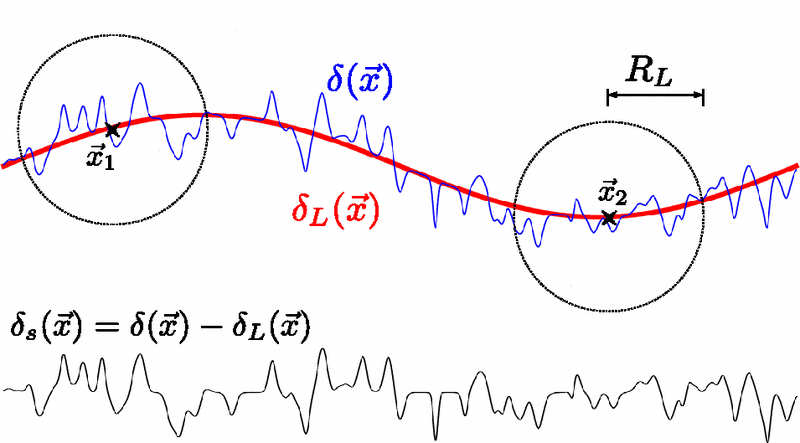
\includegraphics[width=\linewidth]{img/PBS}
	\textcolor{gray}{\fontsize{5.5}{10}\selectfont Image credit: \href{https://link.aps.org/accepted/10.1103/PhysRevD.88.023515}{F. Schmidt, et al.}}	
}
\begin{align*}
	\uncover<+->{
		&\delta(\vec{x}) \equiv \delta_L(\vec{x}) + \delta_s(\vec{x})
		\uncover<2->{,\quad\delta(\vec{x}) = \frac{\rho(\vec{x}) - \rho_c}{\rho_c}}\\~\\
	}
	\uncover<4->{
		&\delta_L(\vec{x}; R_L) = \int \der^2 \vec{x}^\prime \delta(\vec{x}) W_L(\vec{x} + \vec{x}^\prime; R_L)
	}
\end{align*}
\end{column}
\begin{column}{0.5\linewidth}
\centering
\uncover<5->{
	\vskip 10pt
	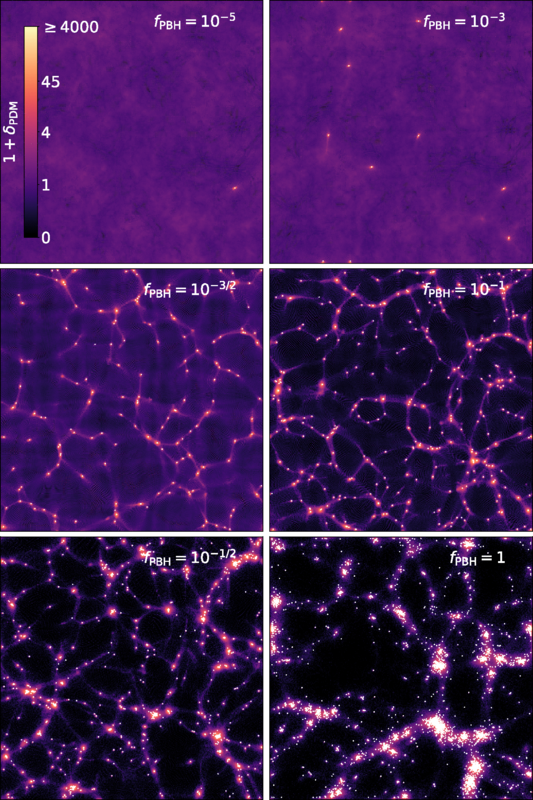
\includegraphics[height=.86\textheight]{img/PBH_Nbody}\\
	\textcolor{gray}{\fontsize{5.5}{10}\selectfont Image credit: \href{https://journals.aps.org/prd/abstract/10.1103/PhysRevD.100.083528}{D. Inman, et al.}}
}
\end{column}
\end{columns}
\end{frame}


% !TeX root = ../defense.tex

\section{Simulations}
\frame{\sectionpage}

\begin{frame}{Spectral energy density}
\begin{equation*}
	\uncover<+->{
		\Omega_{SGWB} = \Omega_{SGWB} (f, \{\Theta_{\text{source}}, \Theta_{\text{astrophysics}}, \Theta_{\text{cosmology}}, \dots\})
	}
\end{equation*}
~\\
\uncover<+->{Depends on:}
\begin{itemize}[<+->]
	\item Source type, Mass scales, ...
	\item Location of sources, Dynamical enviornments, ...
	\item Cosmology model parameters, Mass function, ...
	\item Other observational or Intermediary effects\\~\\
\end{itemize}
\uncover<+->{Ways to calculate $\Omega_{gw}$:}
\begin{enumerate}[<+->]
	\item \textbf{Analytical approach}: For relatively simple models (e.g. inflationary gravitational waves in $\Lambda CDM$ \textcolor{gray}{\fontsize{7.5}{10}\selectfont [\href{https://www.elsevier.com/books/modern-cosmology/dodelson/978-0-12-815948-4}{Dodelson, Schmidt}]})
	
	\item \textbf{Simulation}: For Complicated models with high accuracy (e.g. \textcolor{gray}{\fontsize{7.5}{10}\selectfont [\href{https://www.sciencedirect.com/science/article/pii/S2212686416300553}{Clesse, et al.}], [\href{https://journals.aps.org/prd/abstract/10.1103/PhysRevD.98.063501}{Jenkins, et al.}]})
	
	\item \textbf{Semi-analytocal approach}: For quickly testing various complicated models whithout using too much computational resource (e.g. 
	\textcolor{gray}{\fontsize{7.5}{10}\selectfont [\href{https://iopscience.iop.org/article/10.1088/1475-7516/2021/12/012/meta}{Braglia, et al.}], [\href{https://iopscience.iop.org/article/10.1088/1742-6596/222/1/012021/meta}{Durrer}],
	[\href{https://academic.oup.com/mnras/article-abstract/506/3/3977/6317617}{Mukherjee, et al.}]
	})
\end{enumerate}
\end{frame}

\begin{frame}{Semi-Analytical approach}
\uncover<+->{$\Omega_{SGWB}(f, \{\Theta\}_{i = 0}^n) =$}
$$\uncover<+->{\frac{f}{\rho_c c^2} \int \der^n \Theta_i \int \der z} \uncover<+->{\overbrace{\frac{\der t_r}{\der z}}^{\mathrm{cosmology}}} \uncover<+->{\underbrace{\frac{\der^m \tau_{\text{merg}}(z, \Theta_j)}{\der \Theta_0 \der \Theta_1 \dots \der \Theta_m}}_{\mathrm{\shortstack{astrophysics\\ \&~ cosmology}}}} \uncover<+->{\overbrace{\frac{\der E_{\mathrm{GW}}(f_r, \Theta_k)}{\der f_r}}^{\mathrm{GW~source}}}$$\\~\\~\\

\uncover<+->{$f_r = (1+z) f$}
\end{frame}

\begin{frame}{Cosmology part}
	\uncover<1->{The cosmology is encoded in the Hubble parameter which appears in number of events which occur in a comoving volume between the cosmic times $t_r(z)$ and $t_r(z + \der z)$}\\~\\
	$$\uncover<2->{\frac{\mathrm{d}N}{\mathrm{d}z} = \dot{N}} \uncover<1->{\frac{\mathrm{d}t_r}{\mathrm{d}z}} \uncover<2->{= \frac{\dot{N}}{H(z) (1+z)}}$$\\~\\
	$$\uncover<3->{H^2(z) = H_0^2 \left[\Omega_\mathrm{r}(1+z)^4 + (\Omega_\mathrm{DM} + \Omega_\mathrm{b})(1+z)^3 + \Omega_\mathrm{k}(1+z)^2 + \Omega_\Lambda\right]}$$\\~\\
\end{frame}

\begin{frame}{Astrophysics/Cosmology part}
Following the pictrue in \textcolor{gray}{[M. Braglia, J. Garcia-Bellido, and S. Kuroyanagi, “Testing primordial black holes with multi-band observations of the stochastic gravitational wave background”, \href{https://iopscience.iop.org/article/10.1088/1475-7516/2021/12/012/meta}{\textit{Journal of Cosmology and Astroparticle Physics}, vol.2021, no.12, p.012, 2021.}]}\\~\\
\begin{equation*}
\begin{split}
\uncover<+->{\dot{N}}
\uncover<+->{
	=&\frac{\der^2 \tau_{\text{merg}} (z, m_1, m_2, \{\alpha_z, \alpha_c\})}{\der \log_{10} m_1 \der \log_{10} m_2} =
	} \\
\uncover<+->{&\qquad\qquad\qquad\underbrace{R_{\text{clust}} \frac{(m_1 + m_2)^{10/7}}{(m_1 m_2)^{5/7}} \frac{(1+z)^{\alpha_z}}{\left[1 + (M_{tot} / M_\star)\right]^{\alpha_c}}}_{\mathrm{PBH~clustering/binary~formation}}} \uncover<+->{\overbrace{f_{PBH}(m_1)f_{PBH}(m_2)}^{primordial/thermal~evolution}}
\end{split}
\end{equation*}
\end{frame}

\begin{frame}{Merger rate Calculation an PBH mass function}
~\\~\\
\begin{align*}
	\uncover<+->{
		&\frac{\der^2 \tau_{\text{merg}}^{\mathrm{our~model}}(z, m_1, m_2)}{\der \log_{10} m_1 \der \log_{10} m_2} = R_{\text{clust}} \frac{(m_1 + m_2)^{10/7}}{(m_1 m_2)^{5/7}} f_{PBH}(m_1)f_{PBH}(m_2)\\~\\~\\
	}
	\uncover<+->{
		\text{To fix } R_{\text{clust}}:\quad
		&\int \der m_1 \int \der m_2 \frac{\der^2 \tau_{\text{merg}}^{\mathrm{our~model}}(0, m_1, m_2)}{\der \log_{10} m_1 \der \log_{10} m_2} = 38~yr^{-1} Gpc^{-1}\\~\\~\\
	}
	\uncover<+->{
		&f_{PBH} (m, \{\boxed{\sigma_{PBH}}, \mu\}) = F_0 \frac{1}{\sqrt{2\pi} \sigma_{PBH} m} \exp\left[{-\frac{(\log_{10}\frac{m}{\mu})^2}{2 \sigma_{PBH}^2}}\right]\\~\\~\\
	}
\end{align*}
\end{frame}

\begin{frame}{Source part}
\begin{columns}
\begin{column}{0.6\linewidth}
\begin{align*}
\uncover<+->{
	&\frac{\mathrm{d}E_{\mathrm{GW}}(\Theta_i)}{\mathrm{d}f_r} = \frac{(G\pi)^{2/3}\mathcal{M}_c^{3/5}}{3} \mathcal{G}(f_r, \Theta)\\~\\
}
\uncover<+->{
	&\mathcal{M}_c = \frac{(m_1 + m_2)^{3/5}}{(m_1 + m_2)^{1/5}}\\~\\
}
\end{align*}
\begin{equation*}
\uncover<+->{
	\mathcal{G}(f_r) = 
	\begin{cases}
		\uncover<+->{
			f_r^{-1/3} \qquad & f_r < f_{\mathrm{merg}}\\
		}
		\uncover<+->{
			\frac{f_r^{2/3}}{f_{\mathrm{merg}}} \qquad & f_{\mathrm{merg}} \leq f_r < f_{\mathrm{ring}}\\
		}
		\uncover<+->{
			\frac{1}{f_{\mathrm{merg}} f_{\mathrm{ring}}^{4/3}} \left(\frac{f_r}{1 + \left(\frac{f_r - f_{\mathrm{ring}}}{f_w / 2}\right)^2}\right)^2 \qquad & f_{\mathrm{ring}} \leq f_r < f_{\mathrm{cut}}
		}
	\end{cases}
}
\end{equation*}
\end{column}


\begin{column}{0.4\linewidth}
\begin{align*}
\uncover<+->{
	f_x = &\frac{c^3}{\pi G M_{tot}} \left(a_1 \eta^2 + a_2 \eta + a_3\right)\\~\\
}
\uncover<+->{
	&M_{tot} = m_1 + m_2\\~\\
}
\uncover<+->{
	&\eta = \frac{m_1 + m_2}{M_{tot}^2}\\~\\
}
\end{align*}

\end{column}
\end{columns}
\end{frame}

\begin{frame}{From spectral energy density to wave forms}
\begin{columns}
\begin{column}{0.5\linewidth}
\begin{tikzpicture}%[node distance=1em and 2ex,font=\small]
\uncover<+->{
	\node[flowbox,fb-muted] (model) {
		\fbtitle{page 11}%\vphantom{yÖ}
		\nodepart{two}
		\begin{minipage}{0.9\linewidth}
			%\centering
			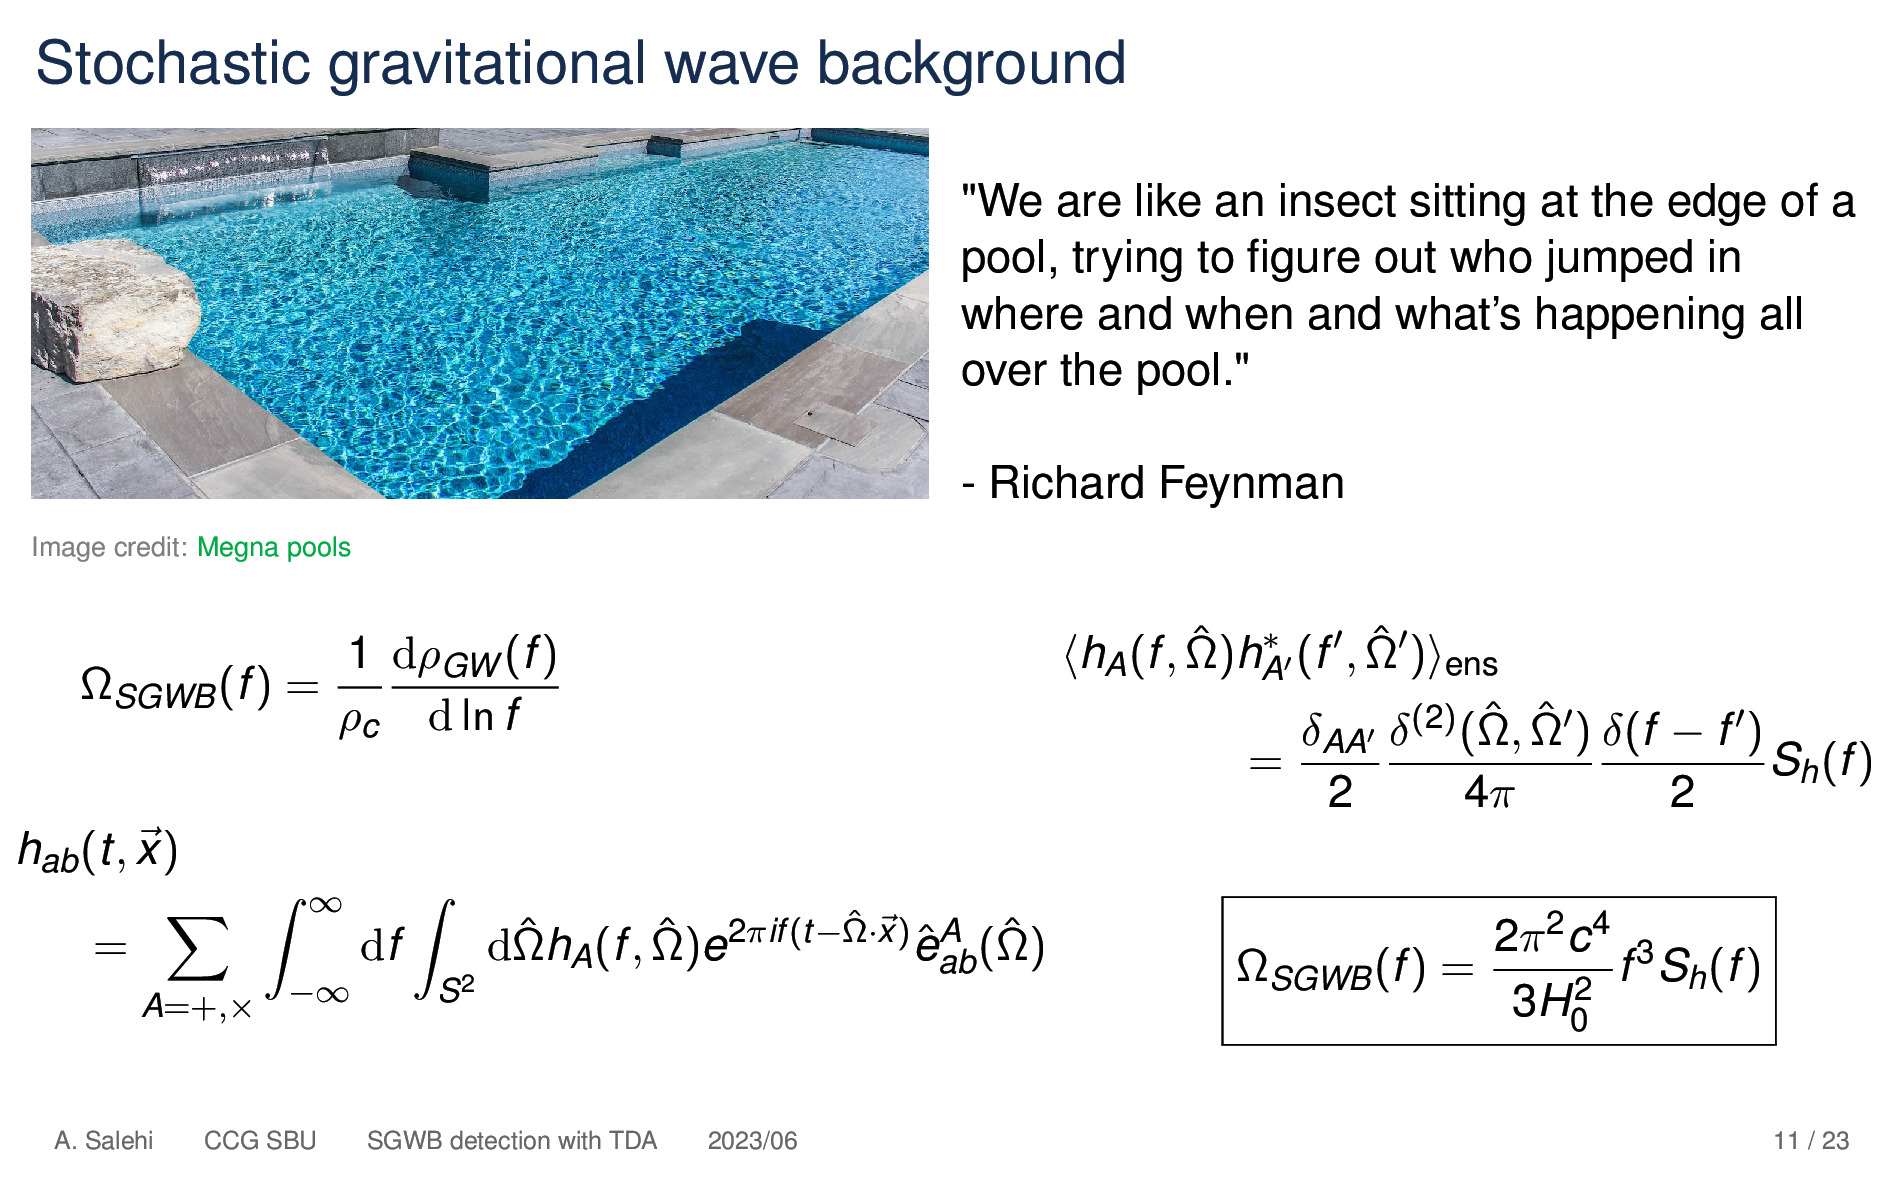
\includegraphics[width=\linewidth]{img/page-11.jpg}
			%\vspace{2ex}
			%\includegraphics[width=.95\textwidth]{img/rivus/scen-today-rivus-networks}
			%\vspace{1ex}
		\end{minipage}
	};
}
\end{tikzpicture}
\end{column}
\begin{column}{0.5\linewidth}
\begin{align*}
\uncover<+->{
	h(t) &= \int_{-\infty}^{\infty} \der f h(f) e^{2 \pi i f (t - \phi)} \\~\\
}
\uncover<+->{
	\langle h(f) h^\star (f^\prime) \rangle &= \frac{\delta (f-f^\prime)}{2} S_h(f) \\
}
\end{align*}
\uncover<+->{To achieve this we used \textit{LALSuite} package with a few added features:}
\begin{itemize}[<+->]
	\item A new data structure to read the numerical spectrum
	\item New functions to simulate SGWB for pawr-law and numerical spectra
	\item Options to access these new functionalities with an app
\end{itemize}
\end{column}
\end{columns}
\end{frame}


\begin{frame}{Spectral energy density plots (theoretical)}
\centering
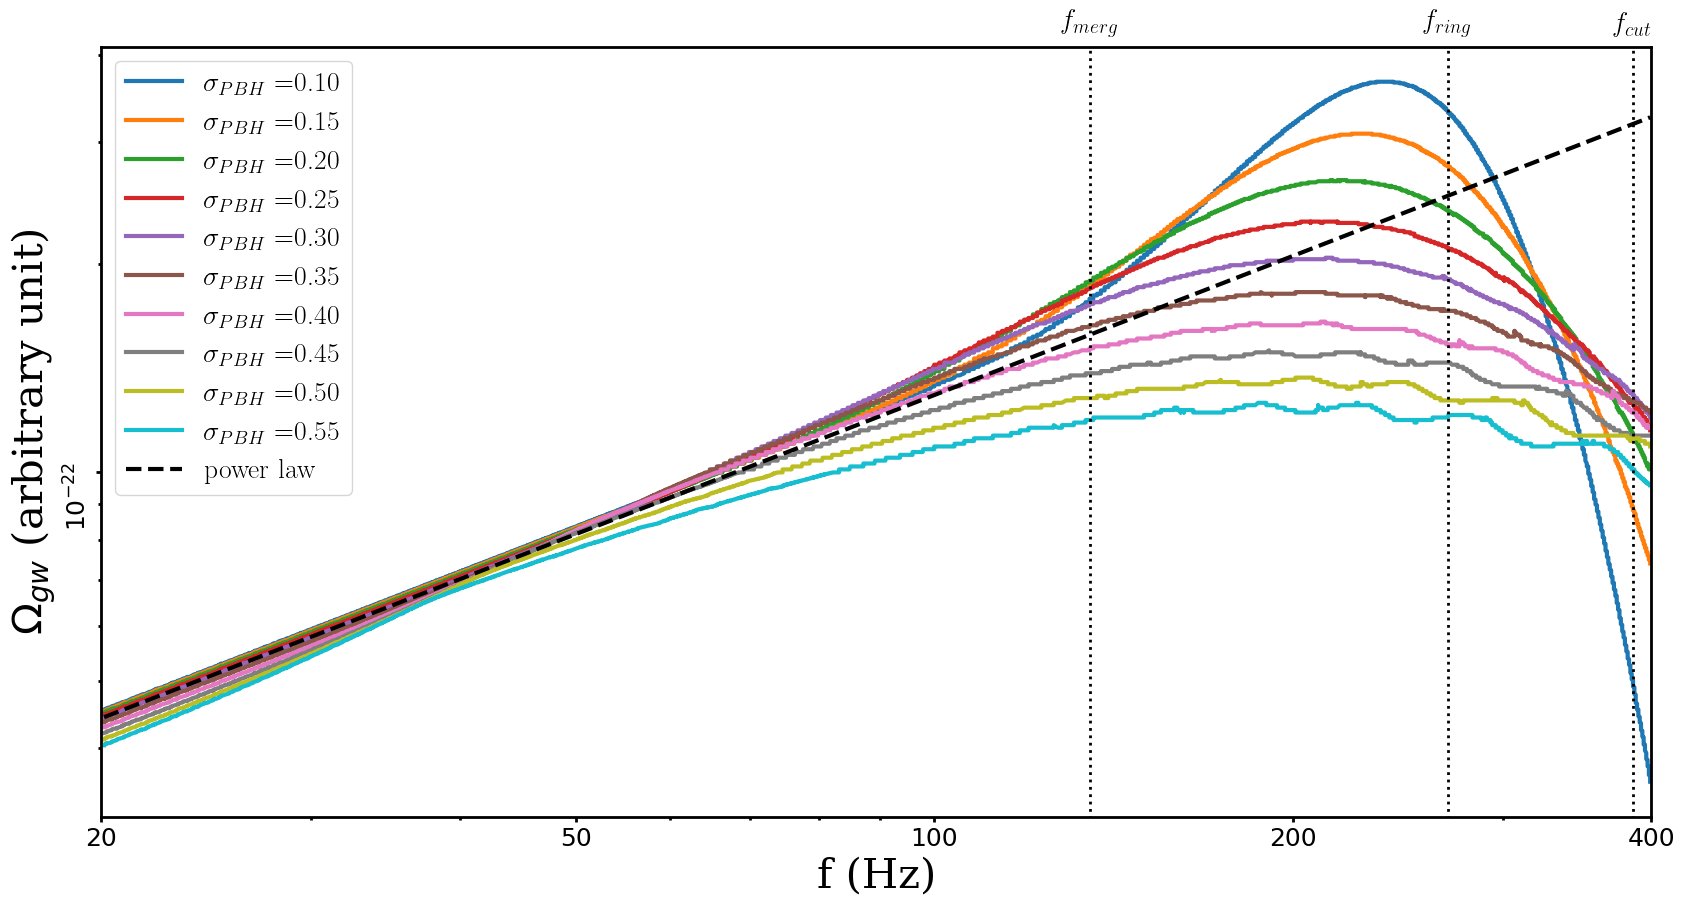
\includegraphics[width=.9\linewidth]{img/theoretical}
\end{frame}

\begin{frame}{Spectral energy density plots (numerical)}
	\centering
	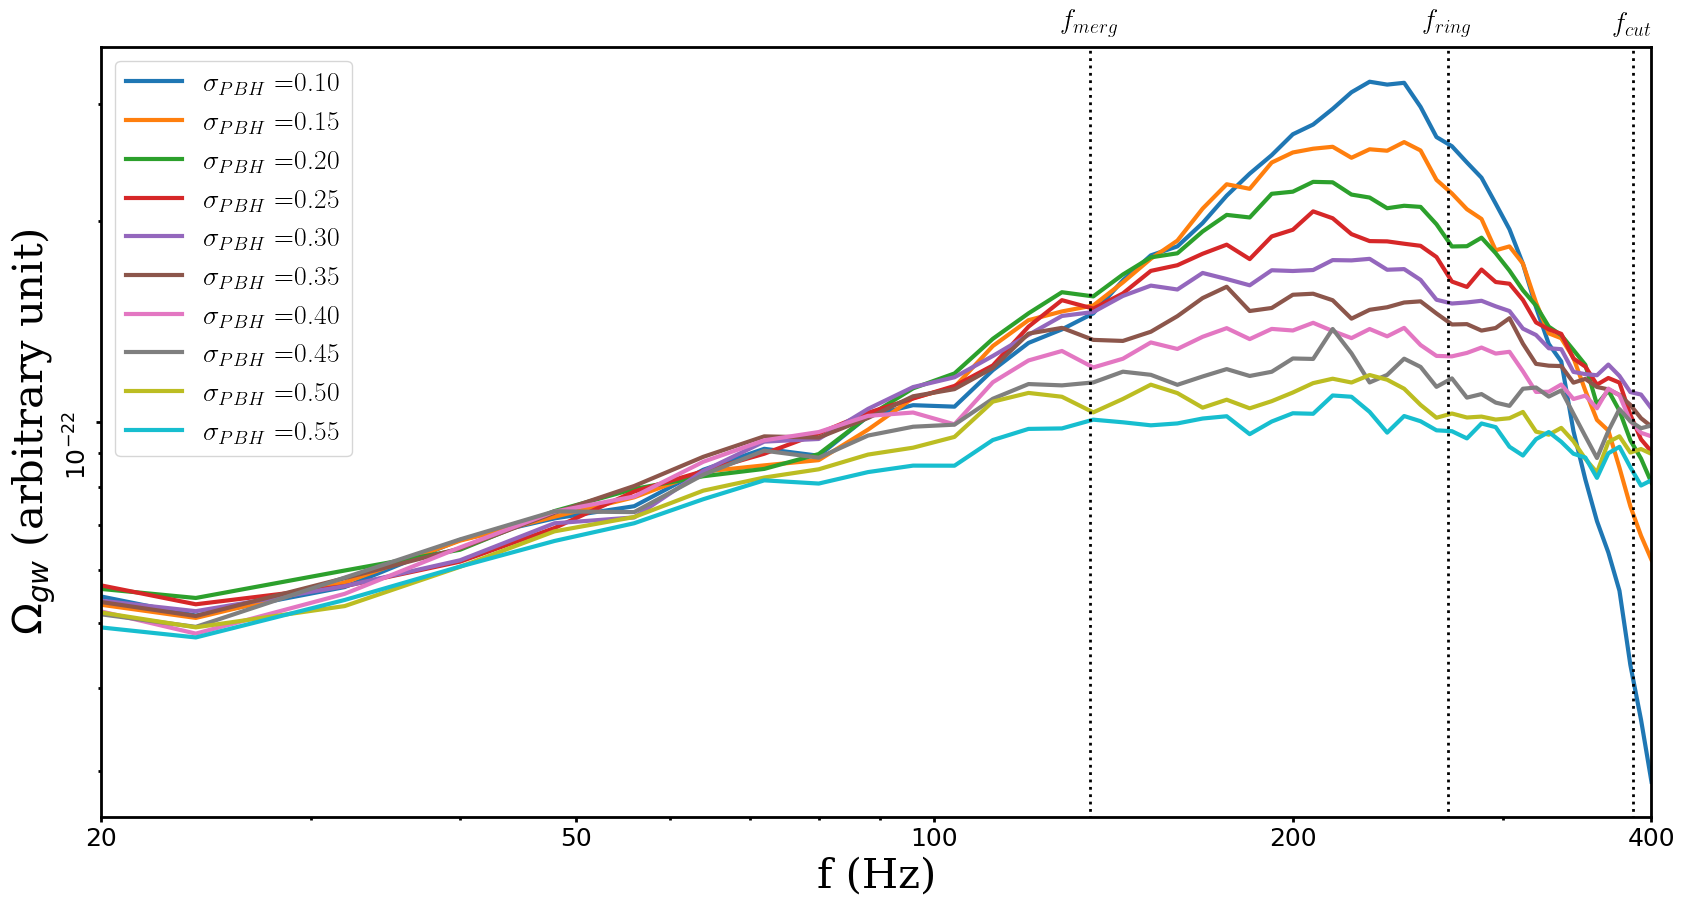
\includegraphics[width=.9\linewidth]{img/numerical}
\end{frame}

\begin{frame}{Spectral energy density plots (noisy)}
	\centering
	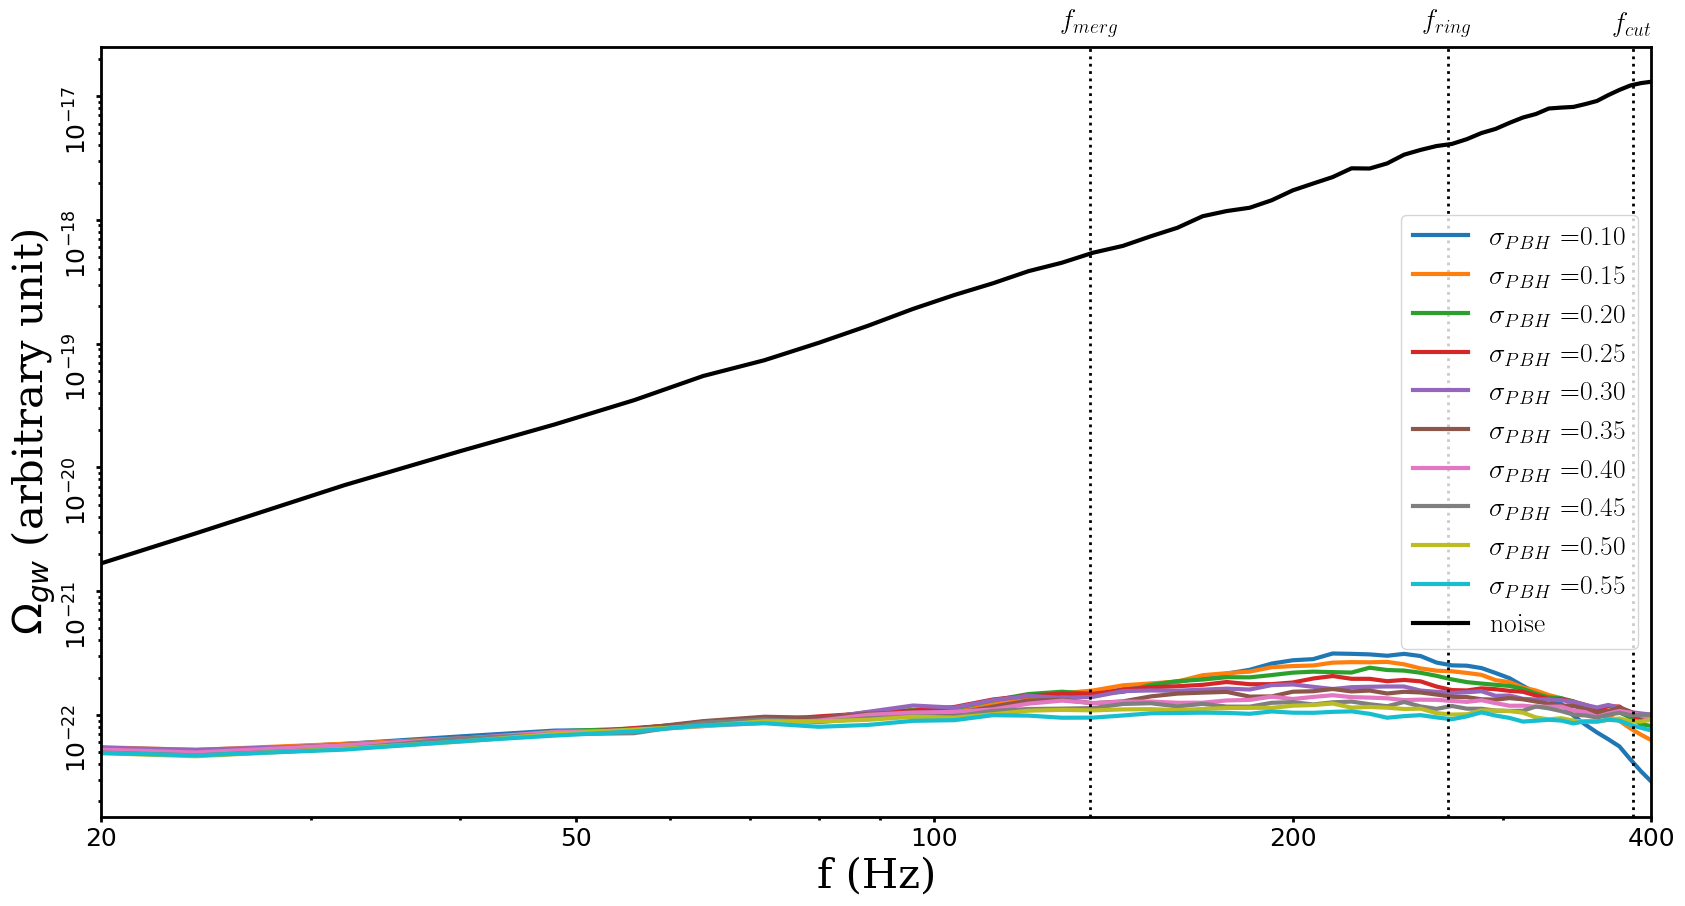
\includegraphics[width=.9\linewidth]{img/noisy}
\end{frame}

\begin{frame}{Recap}
	\uncover{We want to detect:}
	\begin{itemize}
		\item A stochastic gravitational wave background
		\item Coming from binary black hole mergers
		\item Our chosen black holes to study have a primordial origin
	\end{itemize}
	\vskip 1cm
	\uncover{To achieve these, we need:}
	\begin{enumerate}
		\item \sout{Learn about primordial black holes and their population statistics}
		\item \sout{Build a model for their merger rates based on the population statistics}
		\item \sout{Simulate a stochastic gravitational wave background}
		\item Build a model to analyse the data
		\item Run the analyses
	\end{enumerate}
\end{frame}
% !TeX root = ../defense.tex

\section{Topological Data Analysis}
\frame{\sectionpage}

\begin{frame}{What is topology?}
\begin{columns}
\begin{column}{0.6\linewidth}
\uncover<+->{
	\centering
	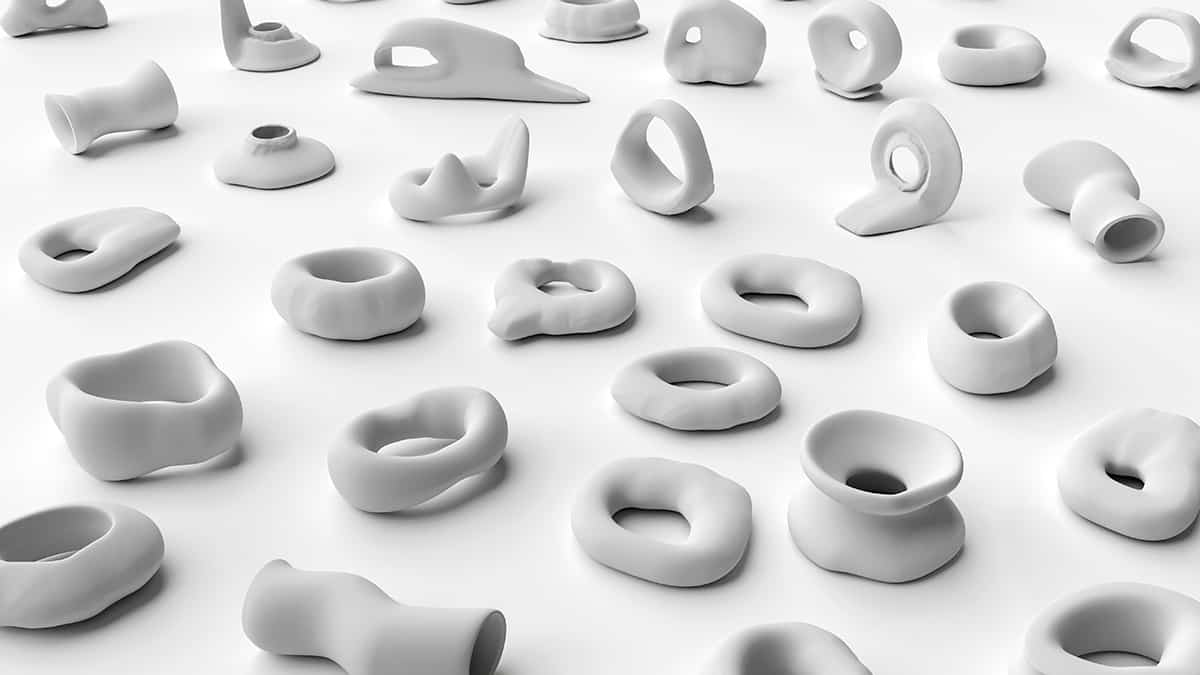
\includegraphics[width=\linewidth]{img/Topological_homeomorphism}\\
	\textcolor{gray}{\fontsize{6.5}{10}\selectfont Image credit: \href{https://physicsworld.com/a/its-topology-naturally/}{Physics world}}
}
\end{column}
\begin{column}{0.4\linewidth}
\uncover<+->{Topology:}
\begin{itemize}[<+->]
	\item The study of holes
	\item Rubber-sheet geometry\\~\\
\end{itemize}
\uncover<+->{Branches of topology:}
\begin{itemize}[<+->]
	\item General Topology or Point Set Topology
	\item Combinatorial Topology
	\item Differential Topology
	\item \boxed{Algebraic Topology}
\end{itemize}
\end{column}
\end{columns}
\end{frame}

\begin{frame}{Homeomorphism}
\begin{columns}
\begin{column}{0.6\linewidth}
\uncover<+->{
	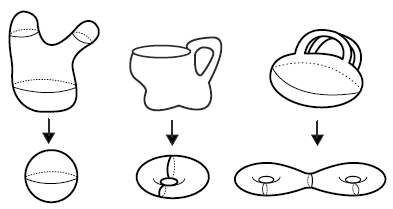
\includegraphics[width=0.6\linewidth]{img/surfaces}\\
	\textcolor{gray}{\fontsize{6.5}{10}\selectfont Image credit: \href{https://uregina.ca/~franklam/Math441_F2019.html}{Annenberg Learner}}\\~\\
}
$\uncover<3->{\beta_k(\psi)} \uncover<4->{= \dim (H_k(\psi))}$\\~\\
\uncover<5->{
	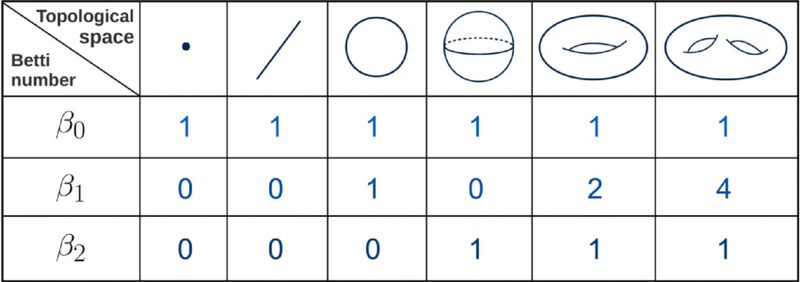
\includegraphics[width=.9\linewidth]{img/betti_numbers}\\
	\textcolor{gray}{\fontsize{6.5}{10}\selectfont Image credit: \href{https://journals.aps.org/pre/abstract/10.1103/PhysRevE.104.034116}{Masoomy, et al.}}
}
\end{column}
\begin{column}{0.4\linewidth}
\uncover<2->{
	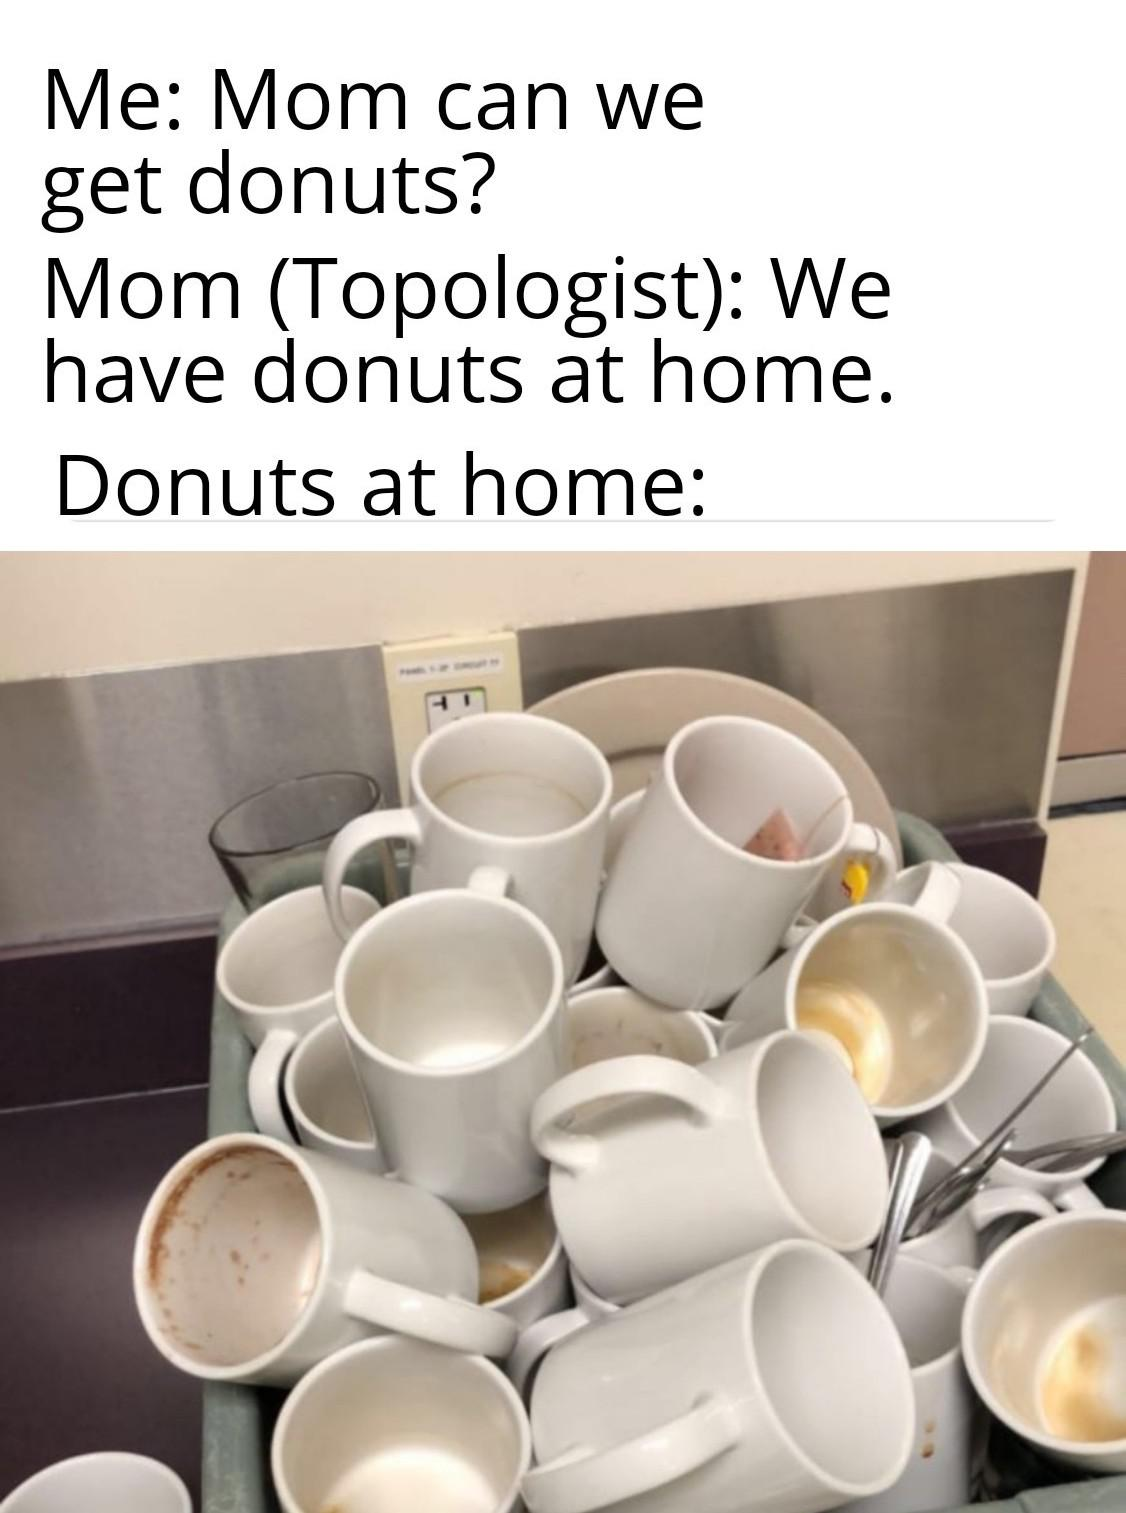
\includegraphics[width=\linewidth]{img/meme}
	\textcolor{gray}{\fontsize{6.5}{10}\selectfont Image source: \href{https://www.reddit.com/r/mathmemes/comments/eilb2c/donuts_at_home/}{Reddit}}
}
\end{column}
\end{columns}
\end{frame}

\begin{frame}{Topology of time series}
\begin{columns}
\begin{column}{0.6\linewidth}
\centering
\uncover<+->{
	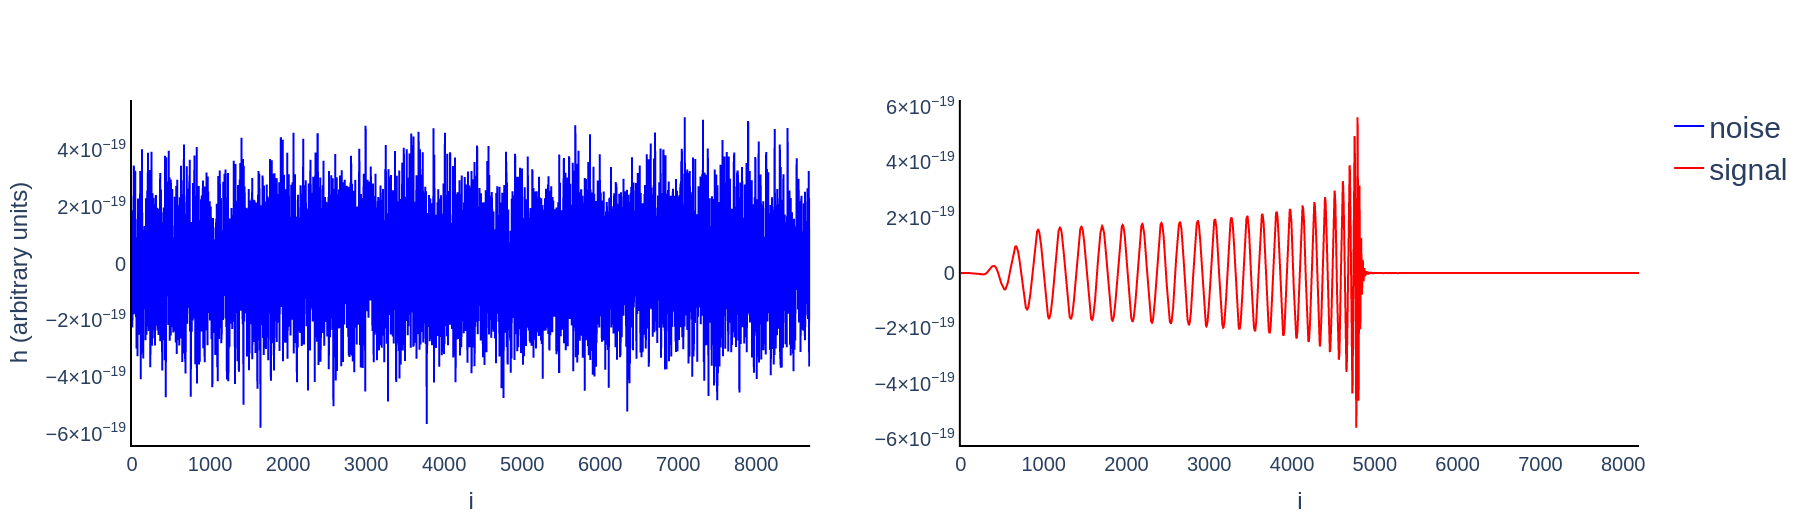
\includegraphics[width=\linewidth]{img/gw_and_noise}
	\\
}
\uncover<6->{
	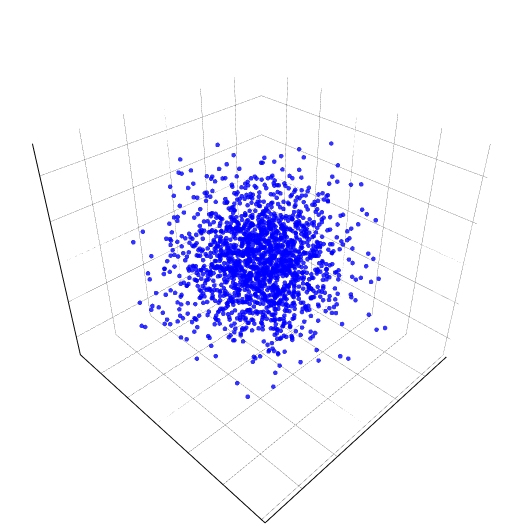
\includegraphics[width=0.35\linewidth]{img/noise_pointcloud}
}
	\hspace{0.1\linewidth}
\uncover<7->{
	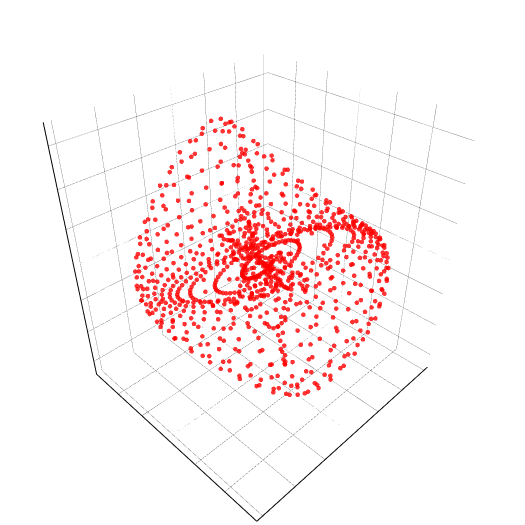
\includegraphics[width=0.35\linewidth]{img/gw_pointcloud}
}
\end{column}
\begin{column}{0.4\linewidth}
\uncover<2->{Taken's embedding:\\}
\begin{align*}
\uncover<3->{x(t) &= (x_1, x_2, \dots, x_i, x_{i+1}, \dots, x_n)}\\
\uncover<4->{t_i &= i \Delta t}\\~\\
\end{align*}

\begin{equation*}
\uncover<5->{
	x(t) \mapsto 
	\begin{pmatrix}
		x_{i} \\
		x_{i + \tau} \\
		\vdots \\
		x_{i + (d-1) \tau}
	\end{pmatrix}
}
\end{equation*}
\end{column}
\end{columns}
\end{frame}

\begin{frame}{Homology theory}
\uncover<+->{In simple terms, homology theory tries to connect the dots in a topological space together and figure out what shape they make\\}
\uncover<+->{To achieve this, homology theory uses \textit{Simplexes} and \textit{Simplical complexes}}
\begin{columns}
\begin{column}{0.4\linewidth}
\vskip .3cm
\centering
\uncover<+->{
	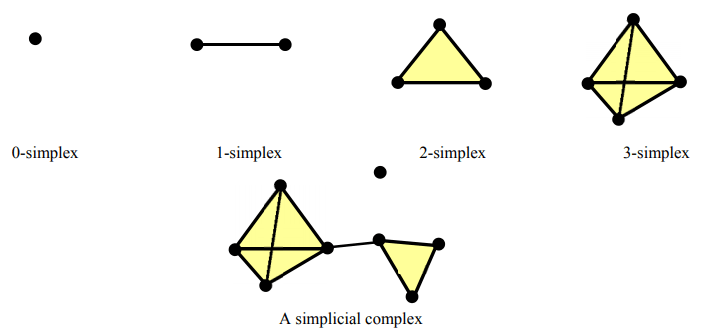
\includegraphics[width=\linewidth]{img/simplicial-complex}\\
	\textcolor{gray}{\fontsize{6.5}{10}\selectfont Image credit: \href{https://aaqr.org/articles/aaqr-18-08-oa-0315}{Zulkepli, et al.}}\\~\\
}
\uncover<4->{
	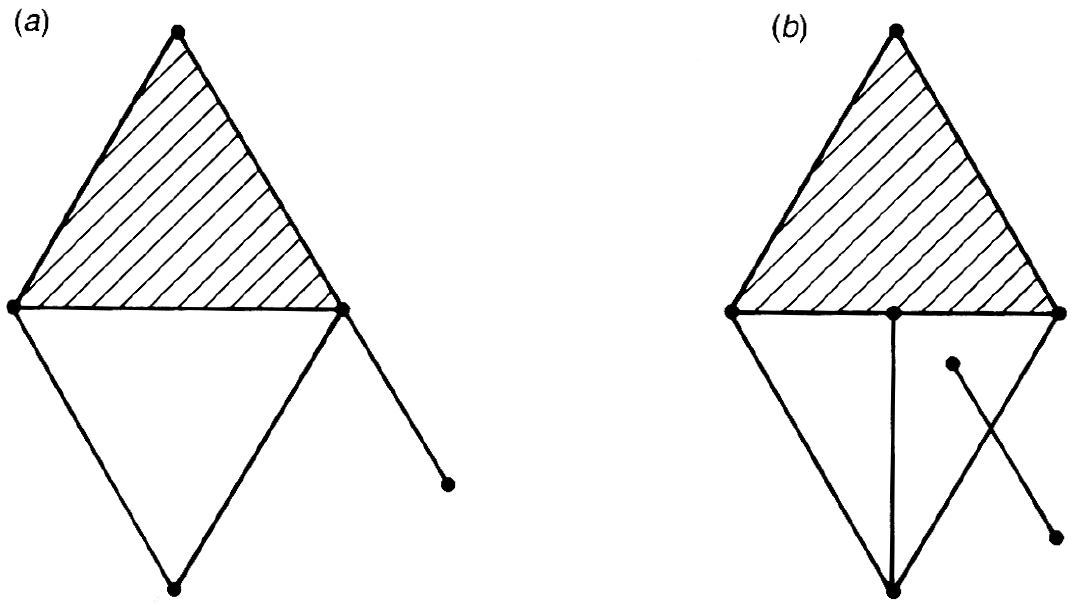
\includegraphics[width=.6\linewidth]{img/complex_not_complex}\\
	\textcolor{gray}{\fontsize{6.5}{10}\selectfont Image credit: \href{https://www.amazon.com/Geometry-Topology-Physics-Graduate-Student/dp/0750306068}{Nakahara}}\\~\\
}
\end{column}
\begin{column}{0.6\linewidth}
\begin{center}

\end{center}
\vskip -.5cm
\uncover<5->{Vietoris-Rips complex}
\begin{align*}
\uncover<6->{
	VR_s(\mathbb{X}) &=\\
	&\left\{\sigma^r = \langle p_0 \dots p_r\rangle ~\bigg\vert~ \forall p_i, p_j \in \sigma^r: ~l^2 (p_i, p_j) \leq s \right\}
}
\end{align*}
\centering
\uncover<7->{
	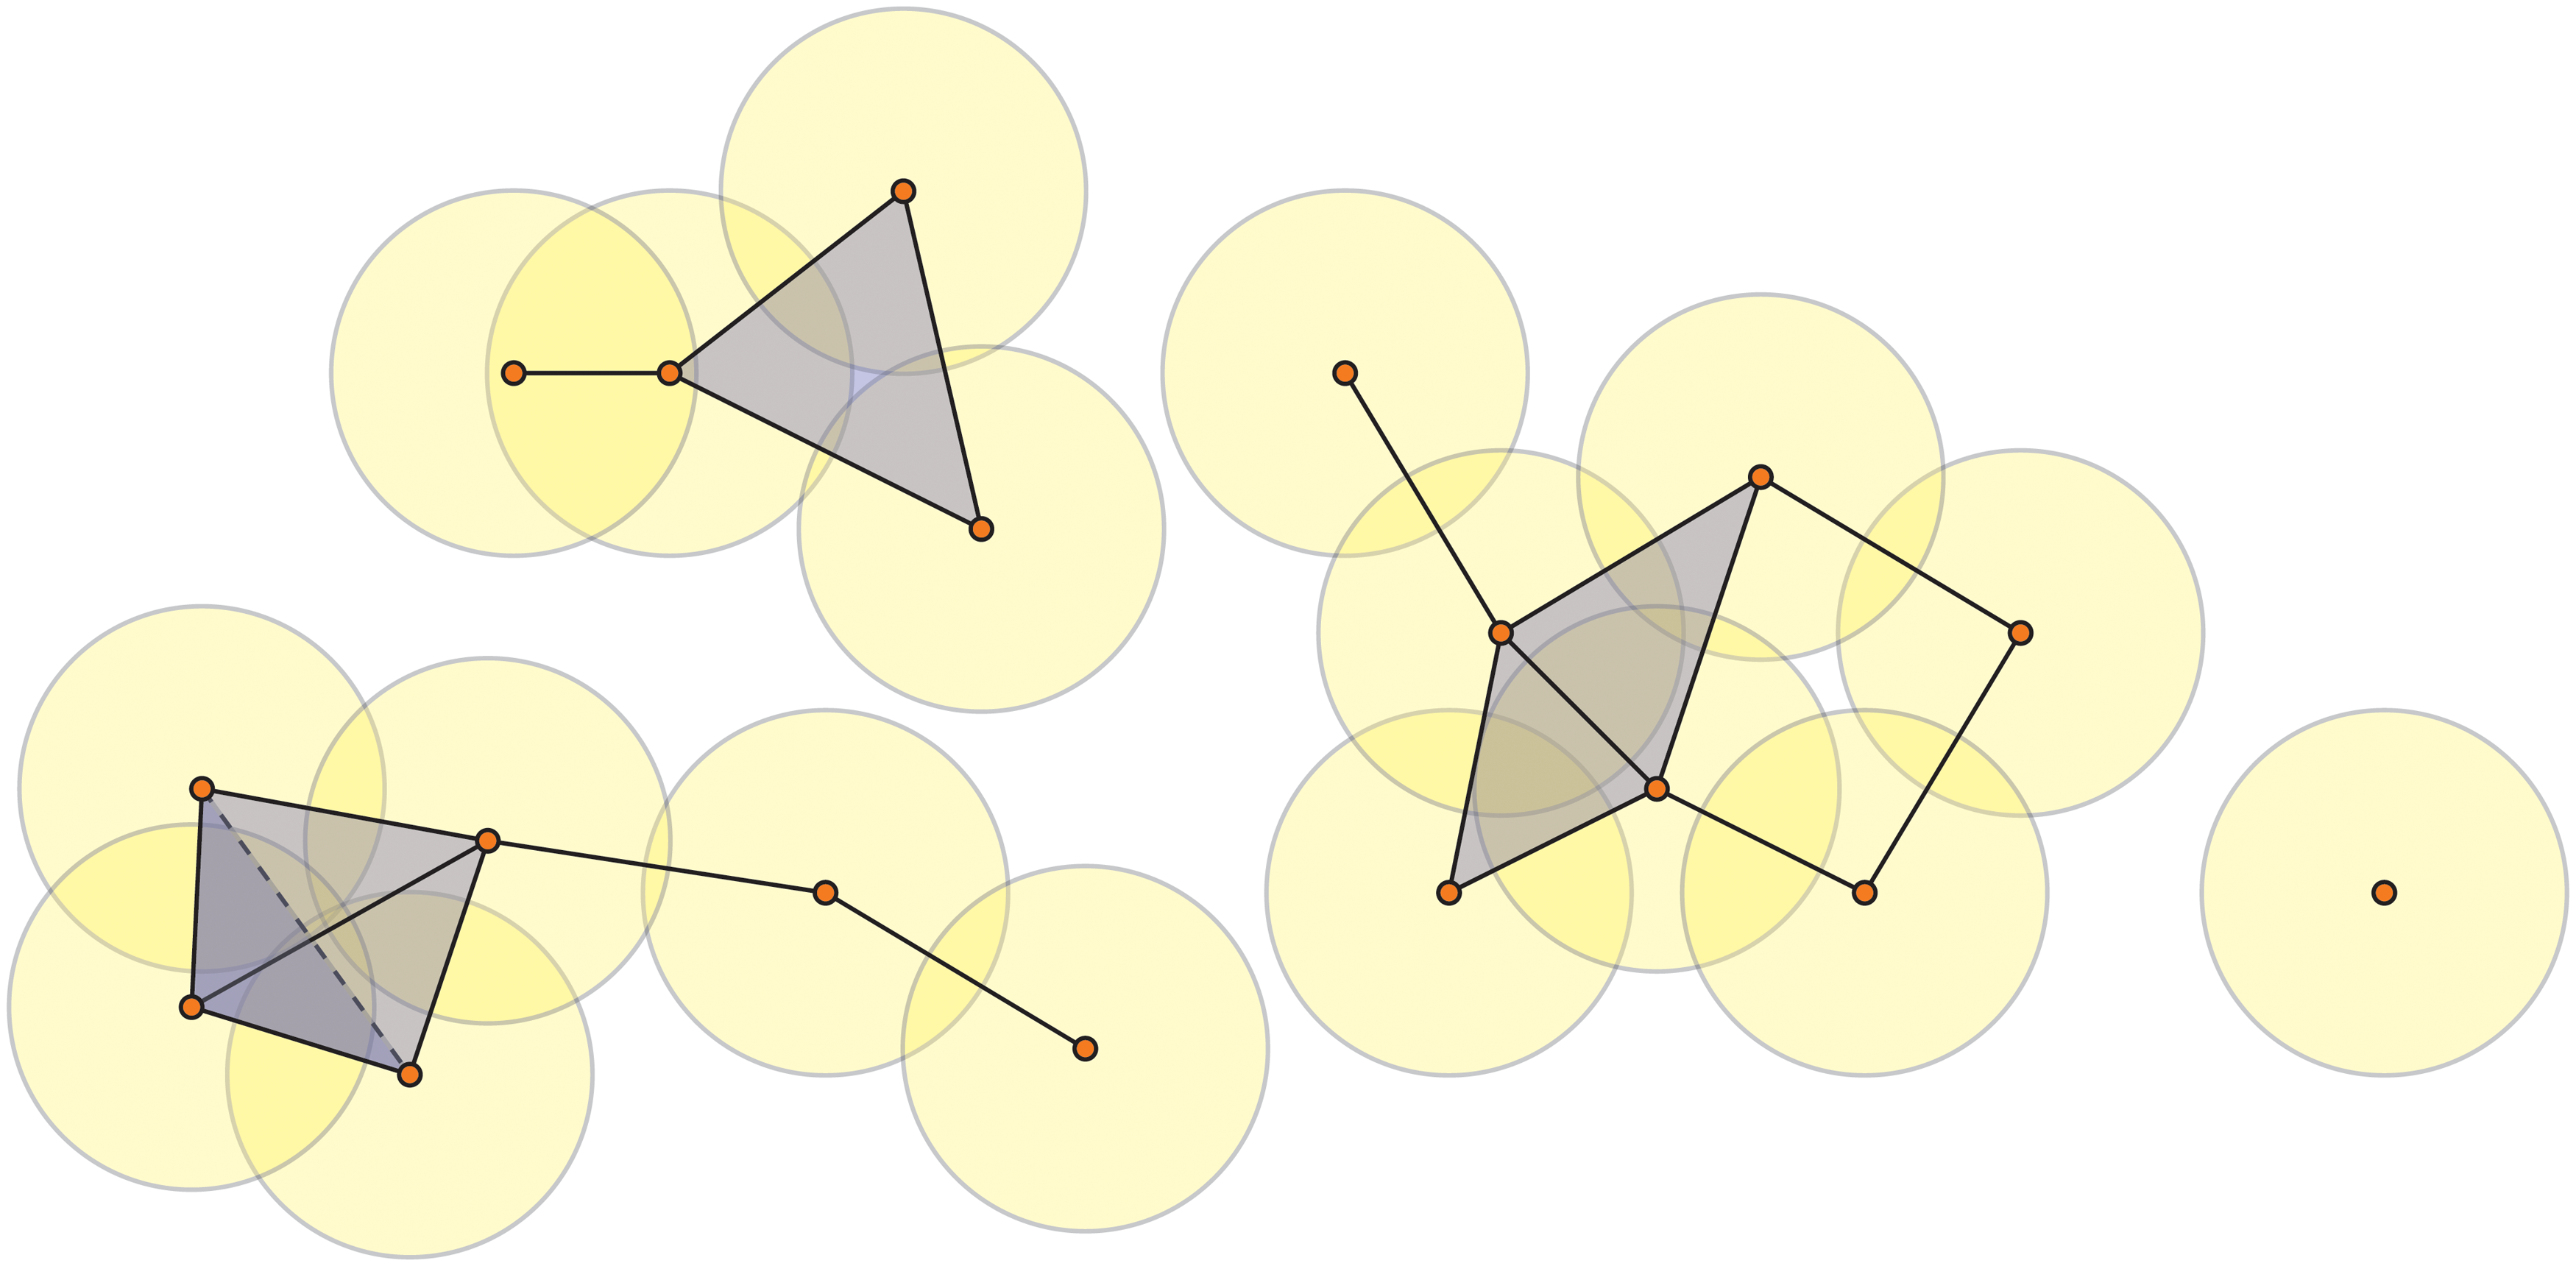
\includegraphics[width=0.75\linewidth]{img/VR_complex}\\
	\textcolor{gray}{\fontsize{6.5}{10}\selectfont Image credit: \href{https://journals.plos.org/plosone/article?id=10.1371/journal.pone.0126383}{Topaz, et al.}}
}
%\vspace*{0.5 cm}
\end{column}
\end{columns}

\end{frame}


\begin{frame}{Persistance homology}
\vskip .5cm
\centering
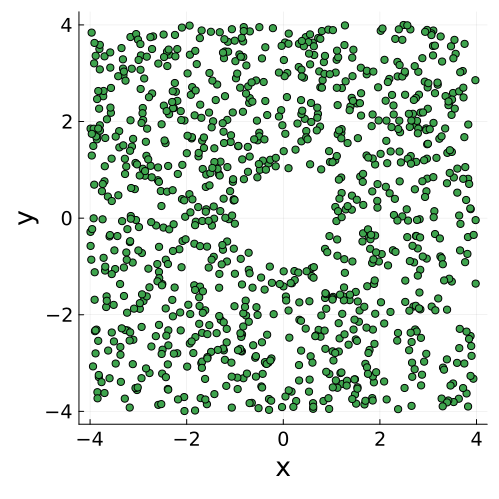
\includegraphics[width=.35\linewidth]{img/cut}
\hspace*{2cm}
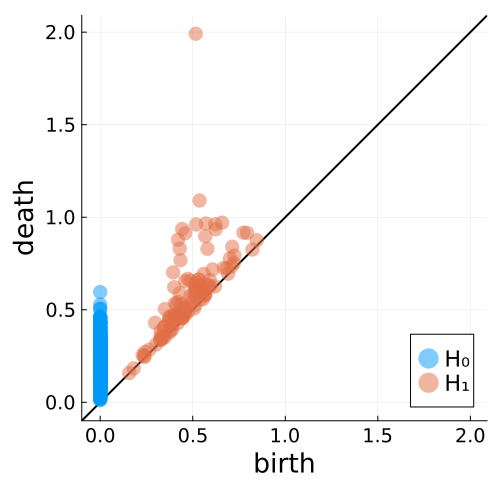
\includegraphics[width=.35\linewidth]{img/PD1}
\uncover<2->{$$\mathbb{X} = \{\mathbb{D}_0, \dots, \mathbb{D}_N\}$$}
\uncover<3->{$$\mathbb{D} = \{(b, d)~\vert~ 0 \leq b < d \in \mathbb{R} \}$$}
\end{frame}

\begin{frame}{Vectorizations and amplitudes}
\begin{columns}
\begin{column}{0.4\linewidth}
\begin{align*}
\uncover<+->{
	&\phi:~ \mathbb{X} \rightarrow \mathbb{V} \\~\\
}
\uncover<+->{
	&A:~ \mathbb{X} \rightarrow \mathbb{R}\\~\\
}
\uncover<+->{
	&A(s) = \vert\vert \phi(s) \vert\vert_p\\~\\
}
\uncover<+->{
	&\vert\vert x \vert\vert_p = (x_1^p + \dots + x_2^p)^{1/p}
}
\end{align*}
\end{column}
\begin{column}{0.6\linewidth}
\vskip -1cm
\centering
\uncover<5->{
	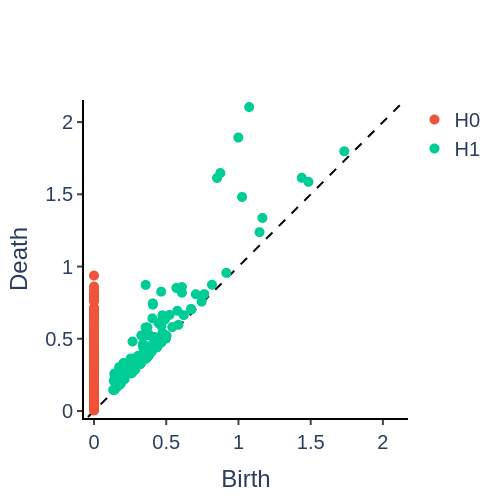
\includegraphics[height=0.35\textheight]{img/PD3.png}
}
\hspace{0.055\textheight}
\uncover<8->{
	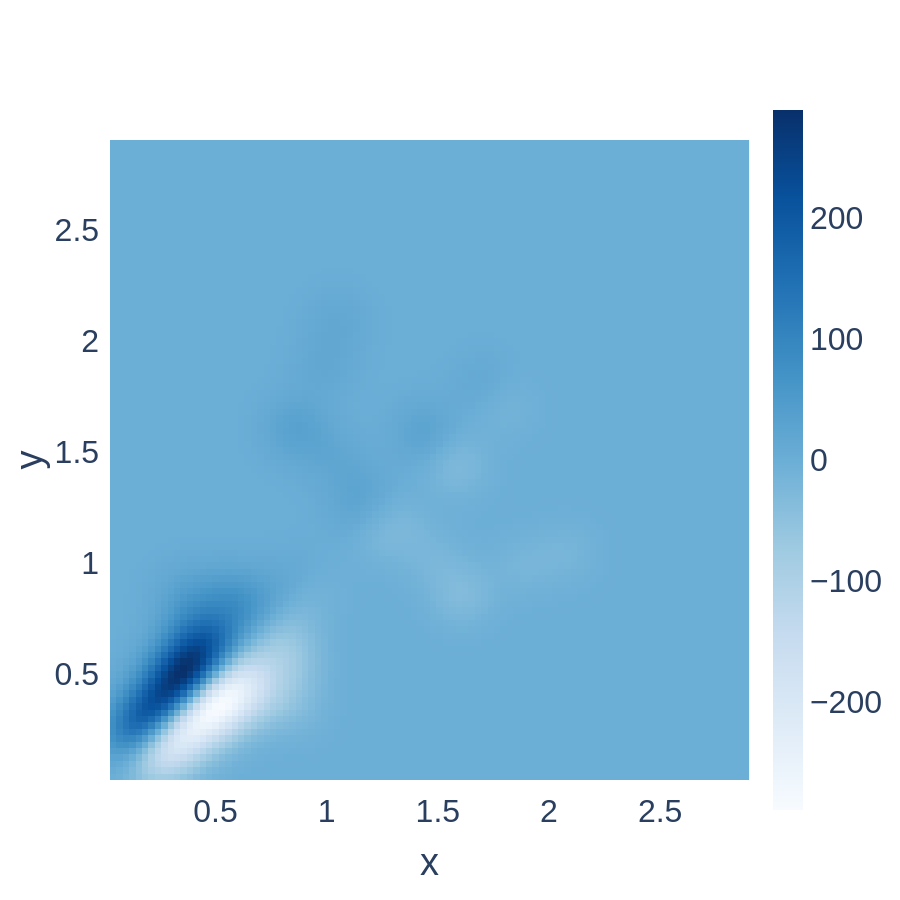
\includegraphics[height=0.35\textheight]{img/HK3.png}
}
\\
\uncover<6->{
	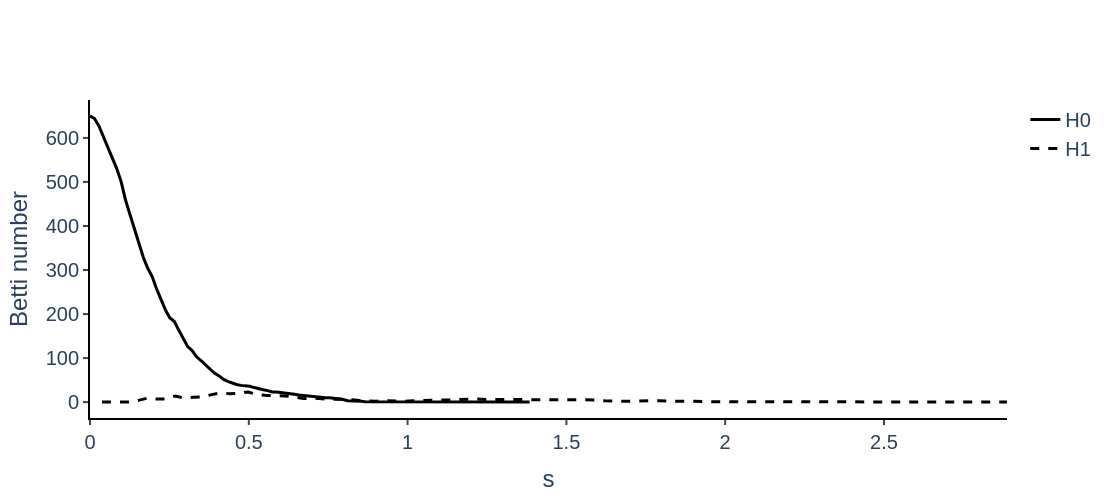
\includegraphics[height=0.35\textheight]{img/BC2.png}
}
\\
\uncover<7->{
	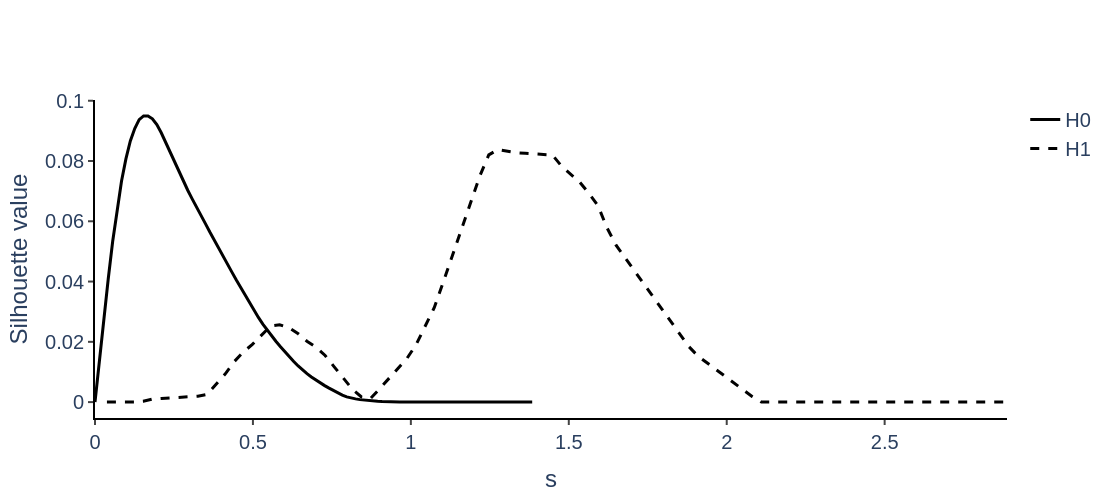
\includegraphics[height=0.35\textheight]{img/SIL2.png}
}
\end{column}
\end{columns}
\end{frame}

\begin{frame}{Recap}
	\uncover<+->{What we have by now:}
	\begin{itemize}[<+->]
		\item A model for primordial black hole binary mergers
		\item A way to simulate a stochastic background based on our model for different population statistics ($\sigma_{PBH}$)
		\item A data analysis method wich has a promise of being resiliant to noise
	\end{itemize}
	\vskip 1cm
	\uncover<+->{Now we are ready to build a data analysis model}\\
	\uncover<+->{We need to:}
	\begin{itemize}[<+->]
		\item Find topological features to detect a signal amidst different levels of noise
		\item Find topological features to discriminate between different values of $\sigma_{PBH}$
		\item A classification method to classify signals with different values of $\sigma_{PBH}$
	\end{itemize}
\end{frame}
% !TeX root = ../defense.tex

\section{Results}
\frame{\sectionpage}

\begin{frame}{Entropy measures}
\centering
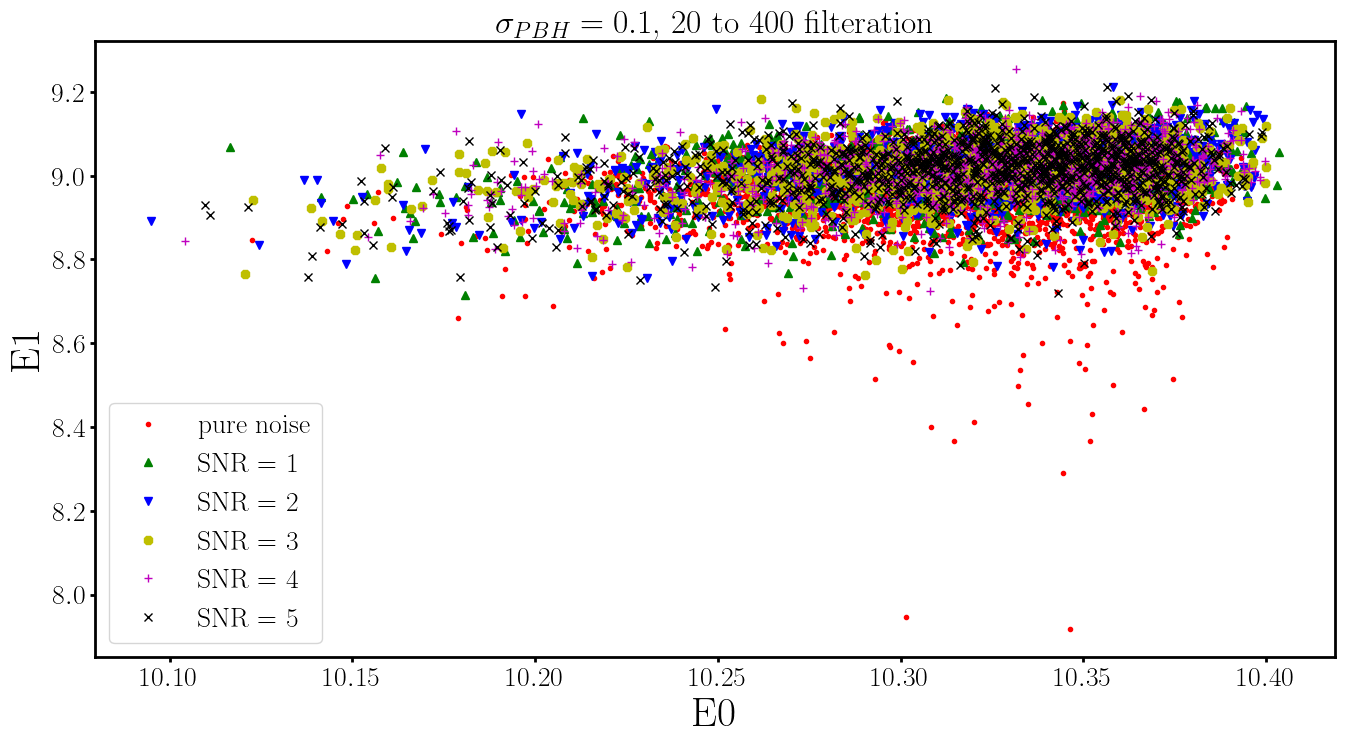
\includegraphics[height=.8\textheight]{img/E0_E1_SNR}
\end{frame}

\begin{frame}{Distance measures}
	\centering
	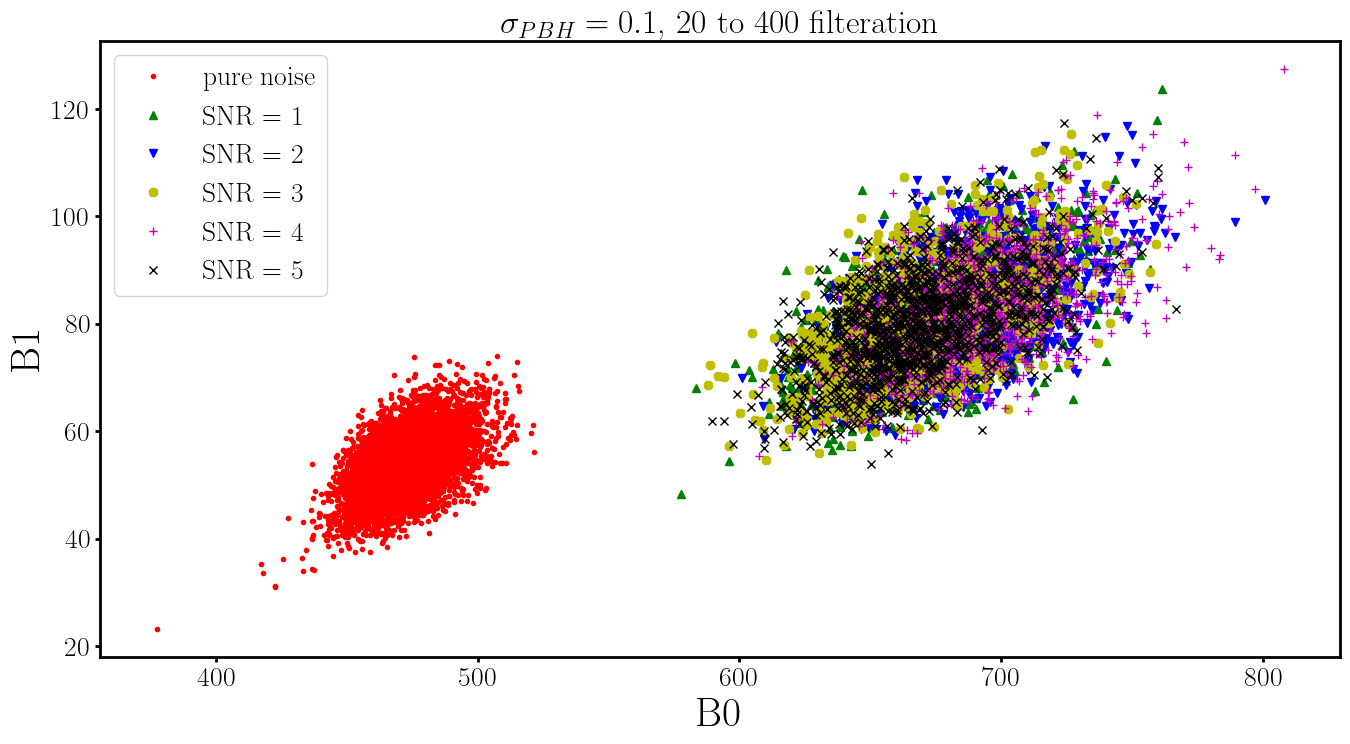
\includegraphics[height=.8\textheight]{img/B0_B1_SNR}
\end{frame}

\begin{frame}{Distance measures}
	\centering
	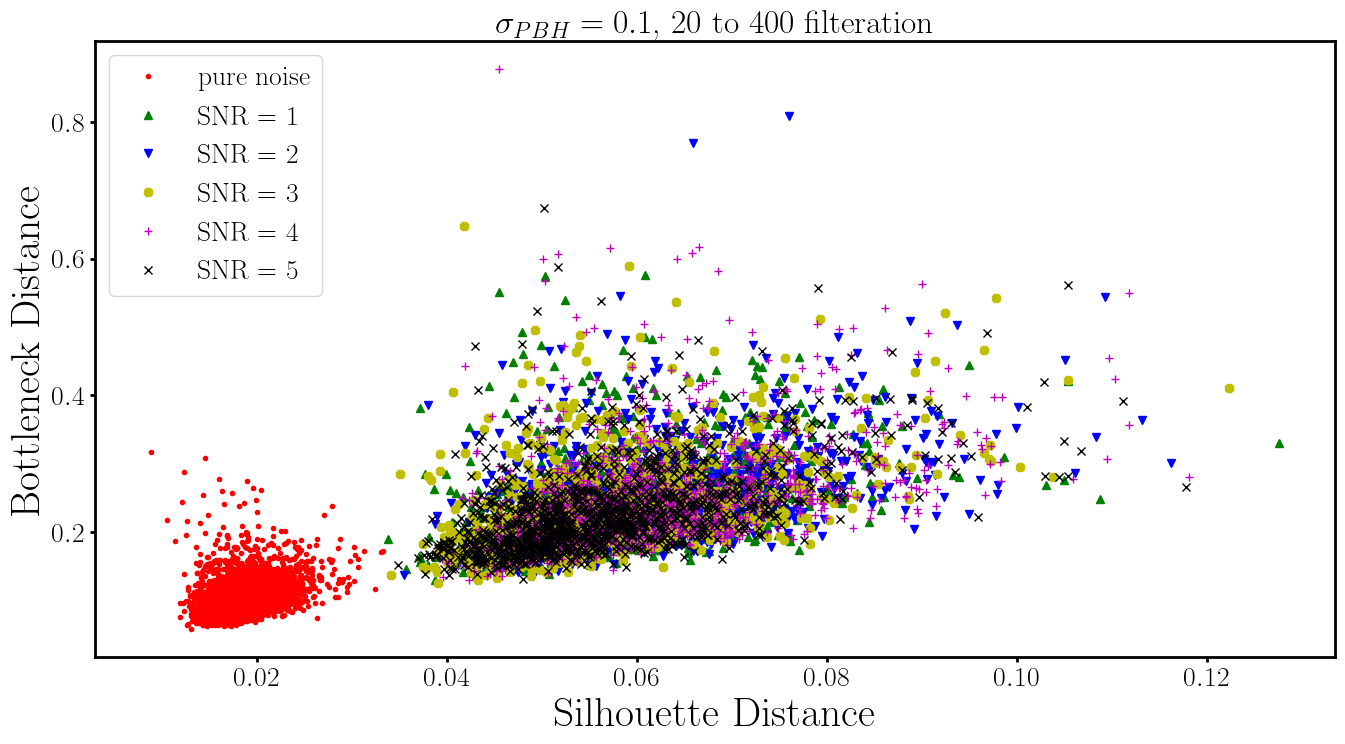
\includegraphics[height=.8\textheight]{img/SD_BD_SNR}
\end{frame}

\begin{frame}{Image measures}
	\centering
	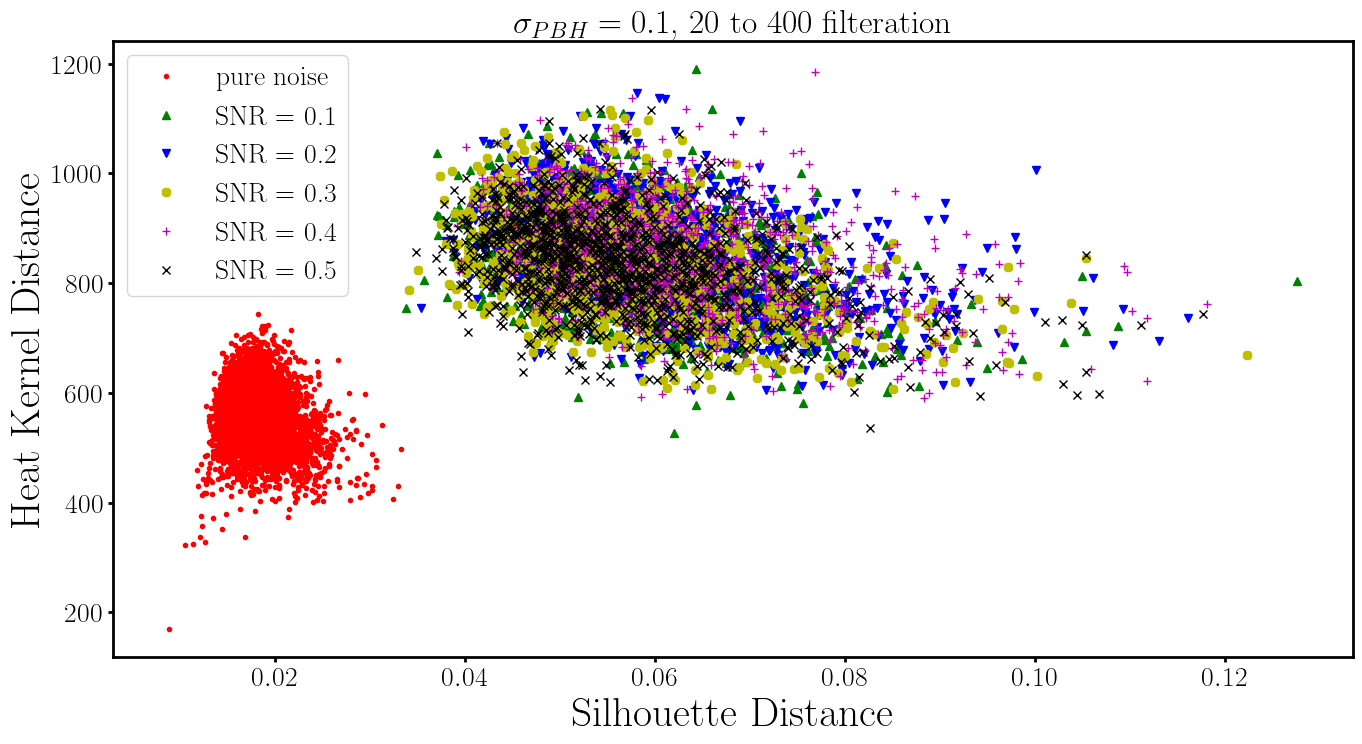
\includegraphics[height=.8\textheight]{img/SD_HK_SNR}
\end{frame}

\begin{frame}{First attempt to classification}
	\centering
	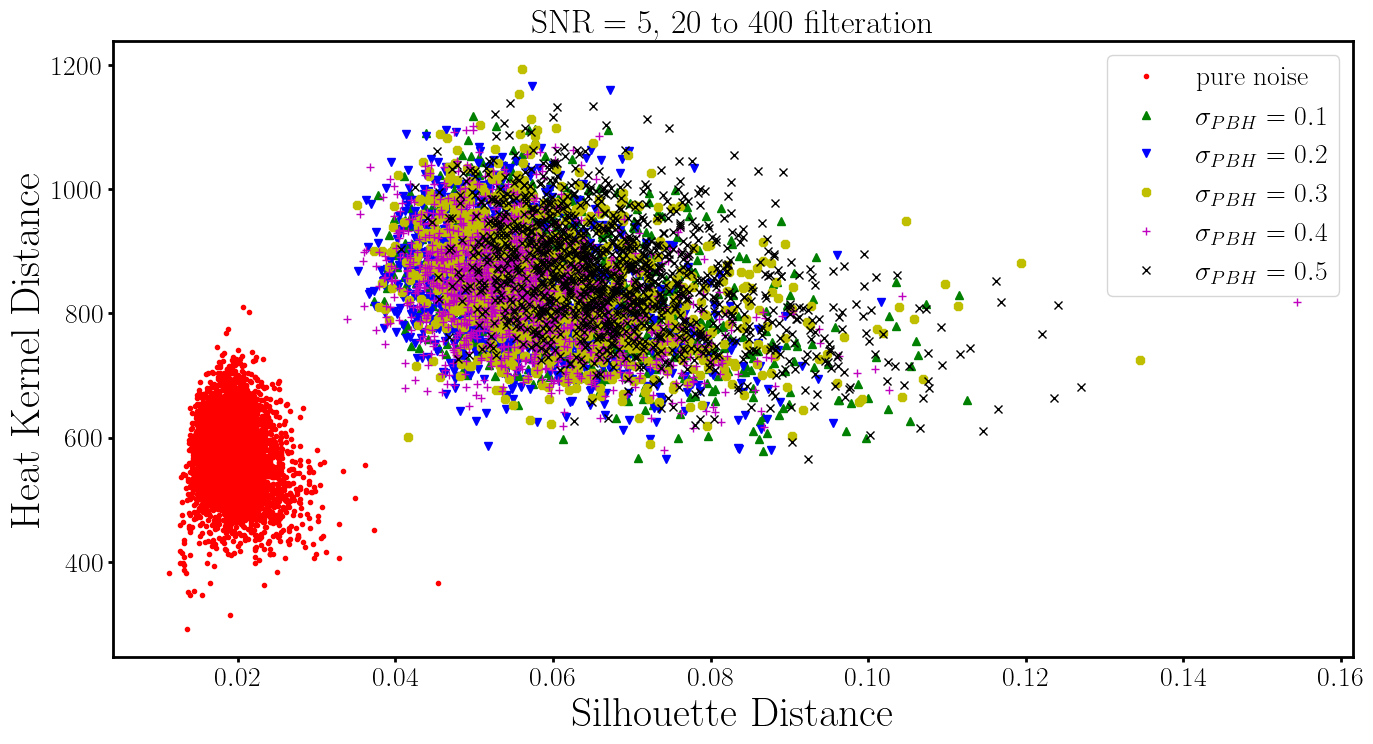
\includegraphics[height=.8\textheight]{img/SD_HK_sig}

\end{frame}

\begin{frame}{What did we learn?}
\begin{enumerate}[<+->]
	\item In contrast to the result from \href{https://arxiv.org/abs/1910.08245}{Bresten and Jung}, entropy measures are not good for detecting a stochastic background.\\~\\
	\item Betti, Silhoutte and Heat Kernel amplitudes when combined together two by two, are very resiliant to noise.\\~\\
	\item The best topological measure to use for detecting the presence of a signal is Betti distance beacuse it's simpler to calculate.\\~\\
	\item Scaler topological measures can not classify the signals based on their physical parameters.\\~\\
\end{enumerate}
\uncover<+->{Hence to build a classification pipeline, we need to use more complicated topological measures.}
\end{frame}

\begin{frame}{A classification pipeline}
	\centering
	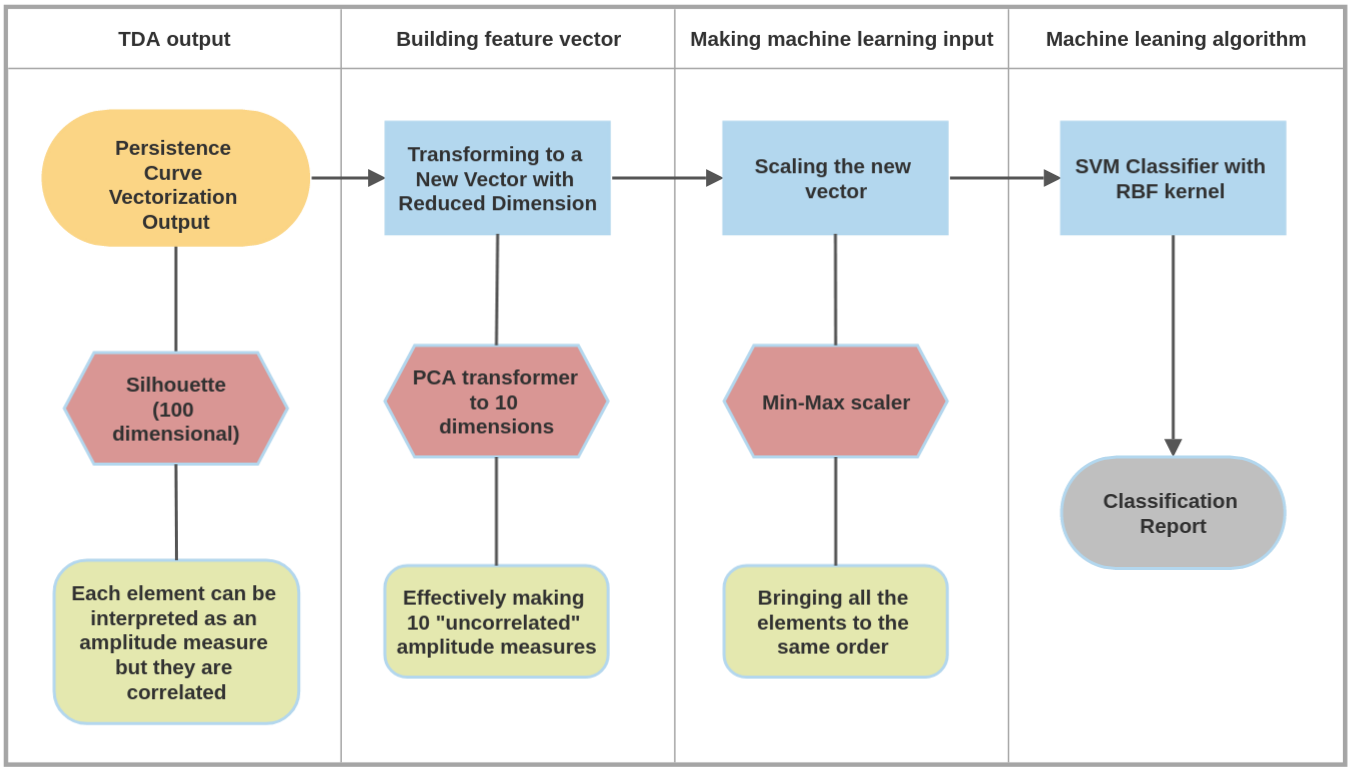
\includegraphics[height=.8\textheight]{img/Classification_algorithm}
\end{frame}

\begin{frame}{Classification report}
\vskip .5cm
\centering
\begin{tabular}{lcccc}
	\textbf{Physical parameter} & \textbf{precision (\%)} & \textbf{recall (\%)} & \textbf{f1-score} & \textbf{support} \\
	\hline \hline
	$\sigma_{PBH}$ = 0.10 & 91 & 85 & 0.88 & 379 \\
	$\sigma_{PBH}$ = 0.15 & 81 & 86 & 0.83 & 345 \\
	$\sigma_{PBH}$ = 0.20 & 93 & 93 & 0.93 & 357 \\
	$\sigma_{PBH}$ = 0.25 & 88 & 94 & 0.91 & 375 \\
	$\sigma_{PBH}$ = 0.30 & 85 & 93 & 0.89 & 328 \\
	$\sigma_{PBH}$ = 0.35 & 95 & 91 & 0.93 & 373 \\
	$\sigma_{PBH}$ = 0.40 & 99 & 97 & 0.98 & 347 \\
	$\sigma_{PBH}$ = 0.45 & 94 & 81 & 0.87 & 366 \\
	$\sigma_{PBH}$ = 0.50 & 89 & 93 & 0.91 & 367 \\
	$\sigma_{PBH}$ = 0.55 & 85 & 87 & 0.86 & 367 \\
	\hline 
	accuracy        &    &    & 0.9 & 3604 \\
	macro avrage    & 90 & 90 & 0.9 & 3604 \\
	\hline \hline
\end{tabular}
\vskip.3cm
\begin{align*}
\uncover<2->{
	\mathrm{precision} = \frac{\mathrm{TP}}{\mathrm{TP} + \mathrm{FP}},\qquad
}
\uncover<3->{
	\mathrm{recall} = \frac{\mathrm{TP}}{\mathrm{TP} + \mathrm{FN}},\qquad
}
\uncover<4->{
	\mathrm{f1-score} = 2 \frac{\mathrm{recall} \times \mathrm{precision}}{\mathrm{recall} + \mathrm{precision}}
}
\end{align*}
\end{frame}
% !TeX root = ../defense.tex

\section{Conclusion and Outlook}
\frame{\sectionpage}

\begin{frame}{Our work in perspective}
\vskip 1cm
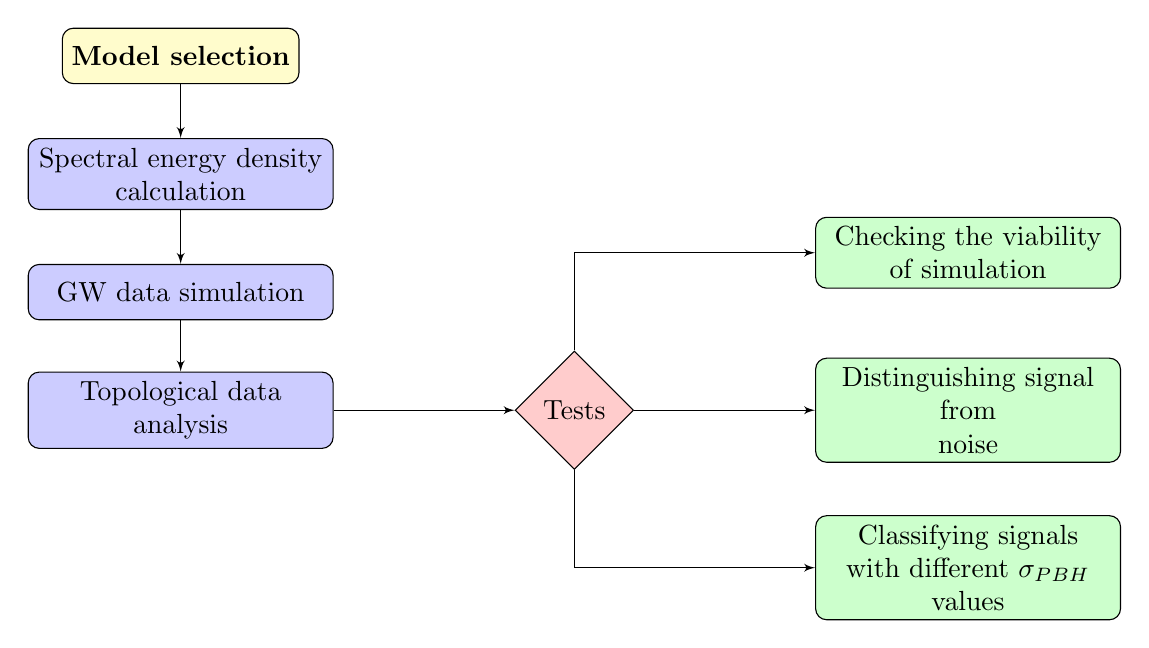
\begin{tikzpicture}
\uncover<+->{
	\node [terminator, fill=yellow!20] at (0,0)  (model)       {\textbf{Model selection}};
}
\uncover<+->{
	\node [terminator, fill=blue!20]   at (0,-1.5) (calculation) {\begin{minipage}{.3\linewidth}
		\centering
		Spectral energy density\\ calculation
	\end{minipage}};
	\path [connector] (model)       -- (calculation);
}
\uncover<+->{
	\node [terminator, fill=blue!20]   at (0,-3) (simulation)  {\begin{minipage}{.3\linewidth}
		\centering
		GW data simulation
	\end{minipage}};
	\path [connector] (calculation) -- (simulation);
}
\uncover<+->{
	\node [terminator, fill=blue!20]   at (0,-4.5) (analysis)    {\begin{minipage}{.3\linewidth}
		\centering
		Topological data analysis
	\end{minipage}};
	\path [connector] (simulation)  -- (analysis);
}
\uncover<+->{
	\node [decision  , fill=red!20]    at (5,-4.5) (tests)       {Tests};
	\path [connector] (analysis)    -- (tests);
}
\uncover<+->{
	\node [terminator, fill=green!20]  at (10,-2.5) (simwork)     {\begin{minipage}{.3\linewidth}
		\centering
		Checking the viability\\ of simulation
	\end{minipage}};
	\path [connector] (tests)       |- (simwork);
}
\uncover<+->{
	\node [terminator, fill=green!20]  at (10,-4.5) (noise)       {\begin{minipage}{.3\linewidth}
		\centering
		Distinguishing signal from\\ noise
	\end{minipage}};
	\path [connector] (tests)       -- (noise);
}
\uncover<+->{
	\node [terminator, fill=green!20]  at (10,-6.5) (class)       {\begin{minipage}{.3\linewidth}
		\centering
		Classifying signals\\ with different $\sigma_{PBH}$ values
	\end{minipage}};
	\path [connector] (tests)       |- (class);
}
\end{tikzpicture}
\end{frame}

\begin{frame}{General statistics}
\uncover<+->{For this work:\\~\\}
\begin{itemize}[<+->]
	\item 3600 signals for 10 different physics were simulated.\\~\\
	\item 6 different noise amplitudes were added.\\~\\
	\item Tens of embedding dimensions and time delays were tested.\\~\\
	\item Tens of topological vectorization and amplitude measures were tested.\\~\\
	\item A 10 dimensional feature vector was selected.\\~\\
	\item A 90\% classification accuracy was achieved.
\end{itemize}
\end{frame}

\begin{frame}{Innovations}
\uncover<+->{Three important innovations were made in this research:\\~\\}
\begin{itemize}[<+->]
	\item A code was written to calculate a spectral energy density using the semi-analytical formula; which is expandable to other astrophysical, cosmological and dynamical scenarios.\\~\\
	\item A number of functions and a data structure were added to the \textit{LALSuite} package which enable it to simulate a SGWB from a custom $\Omega_{SGWB}$.\\~\\
	\item A novel topological measure was introduced which can classify different SGWBs based on their physical parameters.
\end{itemize}
\end{frame}

\begin{frame}{Suggestions}
\uncover<+->{In the future we can expand on this research by doing:\\~\\}
\begin{itemize}[<+->]
	\item A Fischer forcast to evaluate the detection probability of PBH-induced SGWBs via different ovservatories.\\~\\
	\item Comparing our classification results with the results from more classical algorithms.\\~\\
	\item Considering other PBH formation scenarios and simulating their SGWBs.\\~\\
	\item Changing various astrophysical and cosmological parameters to investigate our models ability to constrain those parameters.
\end{itemize}
\end{frame}

\begin{frame}{Accessibility}
In the end, if you are interested in my research, you can sownload my thesis and see my contact information on my page at physics department's computational cosmology group website:
\vskip 2cm
\centering
\LARGE \href{http://ccg.sbu.ac.ir/people/ali-salehi/}{ccg.sbu.ac.ir/people/ali-salehi}
\end{frame}

\usebackgroundtemplate{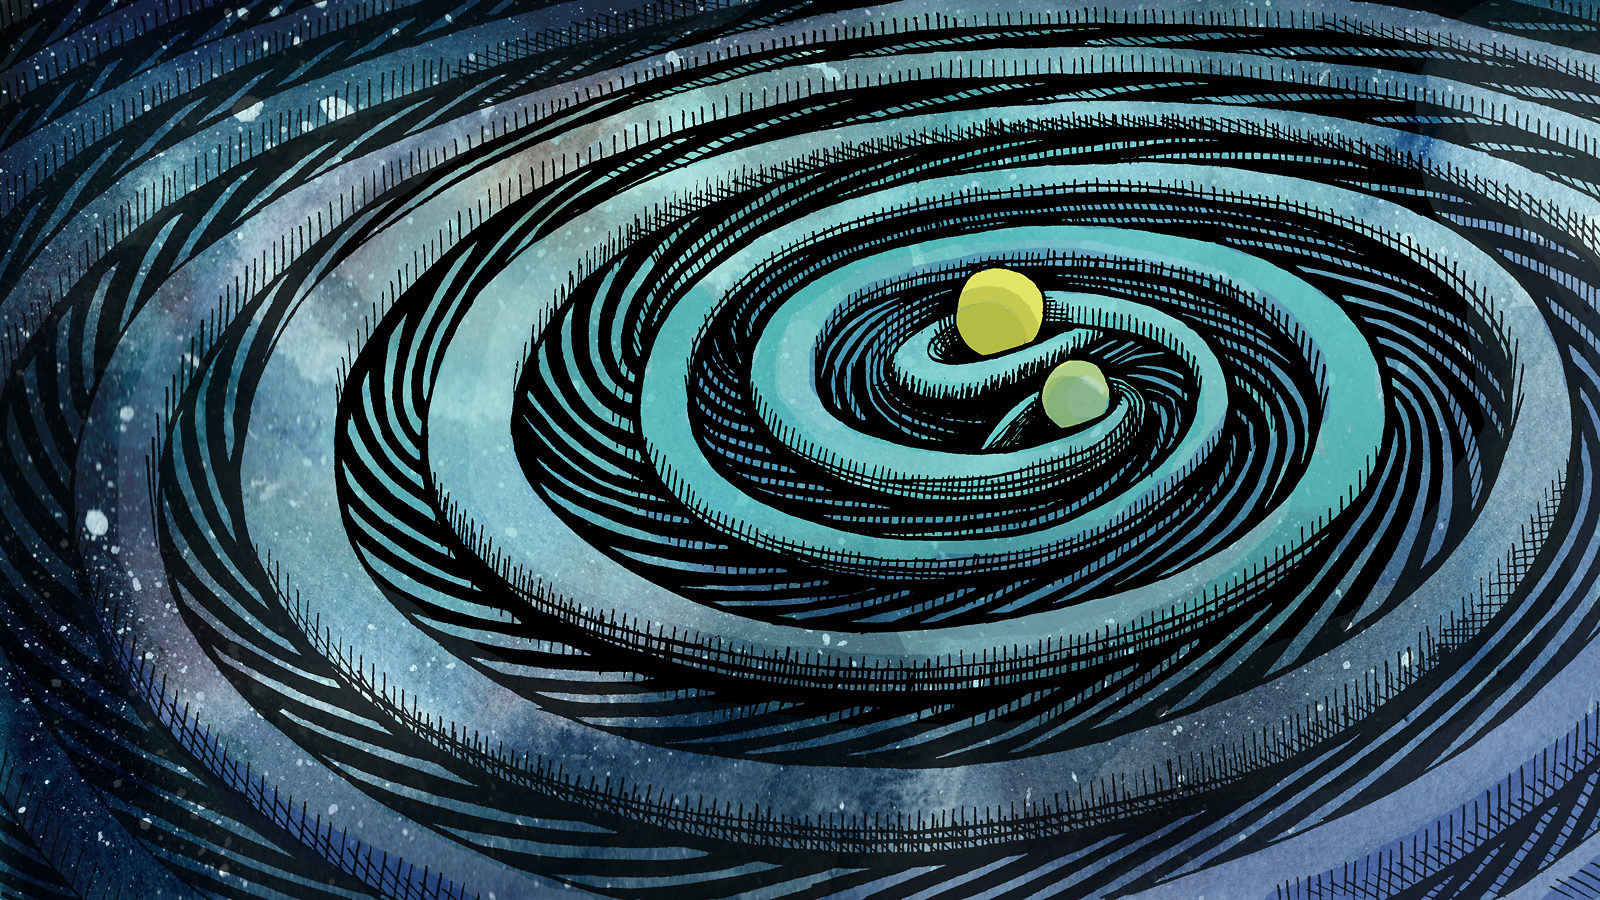
\includegraphics[height=\paperheight]{img/gw-cartoon}}
\begin{frame}[plain]
\begin{center}
\vspace*{5cm}
\contourlength{2pt} %how thick each copy is
\contournumber{20}  %number of copies
\contour{black}{\Huge \textcolor{white}{Thank you for your attention!}}\\
%\Huge \textcolor{white}{Thank you for your attention!}\\
\end{center}
\end{frame}
\end{document}
